
%\documentclass[a4paper,11pt,twoside]{ThesisStyle}
\documentclass[a4paper,11pt,twoside]{article}
\author{M. Hattawy}
\date{\today}
\usepackage{amsmath,amssymb}             % AMS Math
% \usepackage[french]{babel}
\usepackage[latin1]{inputenc}
\usepackage[OT1]{fontenc}
\usepackage[left=2.7cm,right=1.7cm,top=1.6cm,bottom=1.6cm,includefoot,includehead,headheight=13.6pt]{geometry}
\usepackage{setspace}
\usepackage{epigraph}
\usepackage{lineno}


%\usepackage{arev}
%\usepackage[bitstream-charter]{mathdesign}
%\usepackage[urw-garamond]{mathdesign}
%\usepackage[sfmath]{kpfonts} %% sfmath option only to make math in sans serif. Probablye only for use when base font is sans serif.
%\renewcommand*\familydefault{\sfdefault} %% Only if the base font of the document is to be sans serif
\usepackage[sc]{mathpazo}
\linespread{1.05}   
\usepackage[T1]{fontenc}



% Table of contents for each chapter

\usepackage[nottoc, notlof, notlot]{tocbibind}
\usepackage{minitoc}
\setcounter{minitocdepth}{2}
\mtcindent=15pt
% Use \minitoc where to put a table of contents

\usepackage{aecompl}

% Glossary / list of abbreviations

\usepackage[intoc]{nomencl}
\renewcommand{\nomname}{List of Abbreviations}

\makenomenclature

% My pdf code

\usepackage{graphicx,type1cm,eso-pic,color}
\usepackage{lscape}

  \usepackage[pagebackref,hyperindex=true]{hyperref}

%\geometry{letterpaper}
%\graphicspath{{.}{images/}}

% nicer backref links
\renewcommand*{\backref}[1]{}
\renewcommand*{\backrefalt}[4]{%
\ifcase #1 %
(Not cited.)%
\or
(Cited on page~#2.)%
\else
(Cited on pages~#2.)%
\fi}
\renewcommand*{\backrefsep}{, }
\renewcommand*{\backreftwosep}{ and~}
\renewcommand*{\backreflastsep}{ and~}

% Links in pdf
\usepackage{color}
\definecolor{linkcol}{rgb}{0,0,0.4} 
\definecolor{citecol}{rgb}{0.5,0,0} 

% Change this to change the informations included in the pdf file

% See hyperref documentation for information on those parameters

\hypersetup
{
bookmarksopen=true,
pdftitle="",
pdfauthor="", pdfsubject="", %subject of the document
%pdftoolbar=false, % toolbar hidden
pdfmenubar=true, %menubar shown
pdfhighlight=/O, %effect of clicking on a link
colorlinks=true, %couleurs sur les liens hypertextes
pdfpagemode=None, %aucun mode de page
pdfpagelayout=SinglePage, %ouverture en simple page
pdffitwindow=true, %pages ouvertes entierement dans toute la fenetre
linkcolor=linkcol, %couleur des liens hypertextes internes
citecolor=citecol, %couleur des liens pour les citations
urlcolor=linkcol %couleur des liens pour les url
}

% definitions.
% -------------------

\setcounter{secnumdepth}{3}
\setcounter{tocdepth}{2}

% Some useful commands and shortcut for maths:  partial derivative and stuff
\newcommand{\xbp}{$x_{Bj}$}
\newcommand{\xb}{$x_{Bj}~$}
\newcommand{\ptp}{$p_\perp^2$}
\newcommand{\pt}{$p_\perp^2~$}
\newcommand{\dptp}{$\Delta \langle p_\perp^2 \rangle$}
\newcommand{\dpt}{$\Delta \langle p_\perp^2 \rangle ~$}

\brokenpenalty10000\relax

\newcommand{\pd}[2]{\frac{\partial #1}{\partial #2}}
\def\abs{\operatorname{abs}}
\def\argmax{\operatornamewithlimits{arg\,max}}
\def\argmin{\operatornamewithlimits{arg\,min}}
\def\diag{\operatorname{Diag}}
\newcommand{\eqRef}[1]{(\ref{#1})}

\usepackage{rotating}                    % Sideways of figures & tables
%\usepackage{bibunits}
%\usepackage[sectionbib]{chapterbib}          % Cross-reference package (Natural BiB)
%\usepackage{natbib}                  % Put References at the end of each chapter
                                         % Do not put 'sectionbib' option here.
                                         % Sectionbib option in 'natbib' will do.
\usepackage{fancyhdr}                    % Fancy Header and Footer

% \usepackage{txfonts}                     % Public Times New Roman text & math font
  
%%% Fancy Header %%%%%%%%%%%%%%%%%%%%%%%%%%%%%%%%%%%%%%%%%%%%%%%%%%%%%%%%%%%%%%%%%%
% Fancy Header Style Options

\pagestyle{fancy}                       % Sets fancy header and footer
\fancyfoot{}                            % Delete current footer settings

%\renewcommand{\chaptermark}[1]{         % Lower Case Chapter marker style
%  \markboth{\chaptername\ \thechapter.\ #1}}{}} %

%\renewcommand{\sectionmark}[1]{         % Lower case Section marker style
%  \markright{\thesection.\ #1}}         %

\fancyhead[LE,RO]{\bfseries\thepage}    % Page number (boldface) in left on even
% pages and right on odd pages
\fancyhead[RE]{\bfseries\nouppercase{\leftmark}}      % Chapter in the right on even pages
\fancyhead[LO]{\bfseries\nouppercase{\rightmark}}     % Section in the left on odd pages

\let\headruleORIG\headrule
\renewcommand{\headrule}{\color{black} \headruleORIG}
\renewcommand{\headrulewidth}{1.0pt}
\usepackage{colortbl}
\arrayrulecolor{black}

\fancypagestyle{plain}{
  \fancyhead{}
  \fancyfoot{}
  \renewcommand{\headrulewidth}{0pt}
}

%\usepackage{algorithm}
%\usepackage[noend]{algorithmic}

%%% Clear Header %%%%%%%%%%%%%%%%%%%%%%%%%%%%%%%%%%%%%%%%%%%%%%%%%%%%%%%%%%%%%%%%%%
% Clear Header Style on the Last Empty Odd pages
\makeatletter

\def\cleardoublepage{\clearpage\if@twoside \ifodd\c@page\else%
  \hbox{}%
  \thispagestyle{empty}%              % Empty header styles
  \newpage%
  \if@twocolumn\hbox{}\newpage\fi\fi\fi}

\makeatother
 
%%%%%%%%%%%%%%%%%%%%%%%%%%%%%%%%%%%%%%%%%%%%%%%%%%%%%%%%%%%%%%%%%%%%%%%%%%%%%%% 
% Prints your review date and 'Draft Version' (From Josullvn, CS, CMU)
\newcommand{\reviewtimetoday}[2]{\special{!userdict begin
    /bop-hook{gsave 20 710 translate 45 rotate 0.8 setgray
      /Times-Roman findfont 12 scalefont setfont 0 0   moveto (#1) show
      0 -12 moveto (#2) show grestore}def end}}
% You can turn on or off this option.
% \reviewtimetoday{\today}{Draft Version}
%%%%%%%%%%%%%%%%%%%%%%%%%%%%%%%%%%%%%%%%%%%%%%%%%%%%%%%%%%%%%%%%%%%%%%%%%%%%%%% 

\newenvironment{maxime}[1]
{
\vspace*{0cm}
\hfill
\begin{minipage}{0.5\textwidth}%
%\rule[0.5ex]{\textwidth}{0.1mm}\\%
\hrulefill $\:$ {\bf #1}\\
%\vspace*{-0.25cm}
\it 
}%
{%

\hrulefill
\vspace*{0.5cm}%
\end{minipage}
}

\let\minitocORIG\minitoc
\renewcommand{\minitoc}{\minitocORIG \vspace{1.5em}}

\usepackage{multirow}
%\usepackage{slashbox}

\newenvironment{bulletList}%
{ \begin{list}%
	{$\bullet$}%
	{\setlength{\labelwidth}{25pt}%
	 \setlength{\leftmargin}{30pt}%
	 \setlength{\itemsep}{\parsep}}}%
{ \end{list} }

\newtheorem{definition}{D�finition}
\renewcommand{\epsilon}{\varepsilon}

% centered page environment

\newenvironment{vcenterpage}
{\newpage\vspace*{\fill}\thispagestyle{empty}\renewcommand{\headrulewidth}{0pt}}
{\vspace*{\fill}}


\begin{document}

\title{\centering{Follow up on the incoherent t, t'}}
\maketitle

\section{Overview}
In our DVCS analysis, we considered the initial proton of the incoherent 
channel to be at rest, while this is not totally true because of the Fermi 
motion. Does this assumption is a good approximation? What other options can be 
used to minimize this effect on the calculated exclusive quantities?\\

Figure \ref{fig:handbag} presents the leading order handbag diagram of the 
incoherent DVCS channel off $^4$He. Ideally, the transferred momentum squared 
($t$) is defined using the initial and the final nucleons' 4-vectors as 
$(p-p')^{2}$. Then as a DVCS requirement, $t$ has to be greater than a certain 
value ($t_{min}$), which is defined using the kinematics of the incoming and 
the scattered electrons. Due to the knowledge lack of the initial proton's 
momentum, this cut maybe inaccurate, causes loosing some good DVCS events and 
leading to inaccurate determination of the exclusivity cuts.\\ 

\begin{figure}[h!]
\centering
   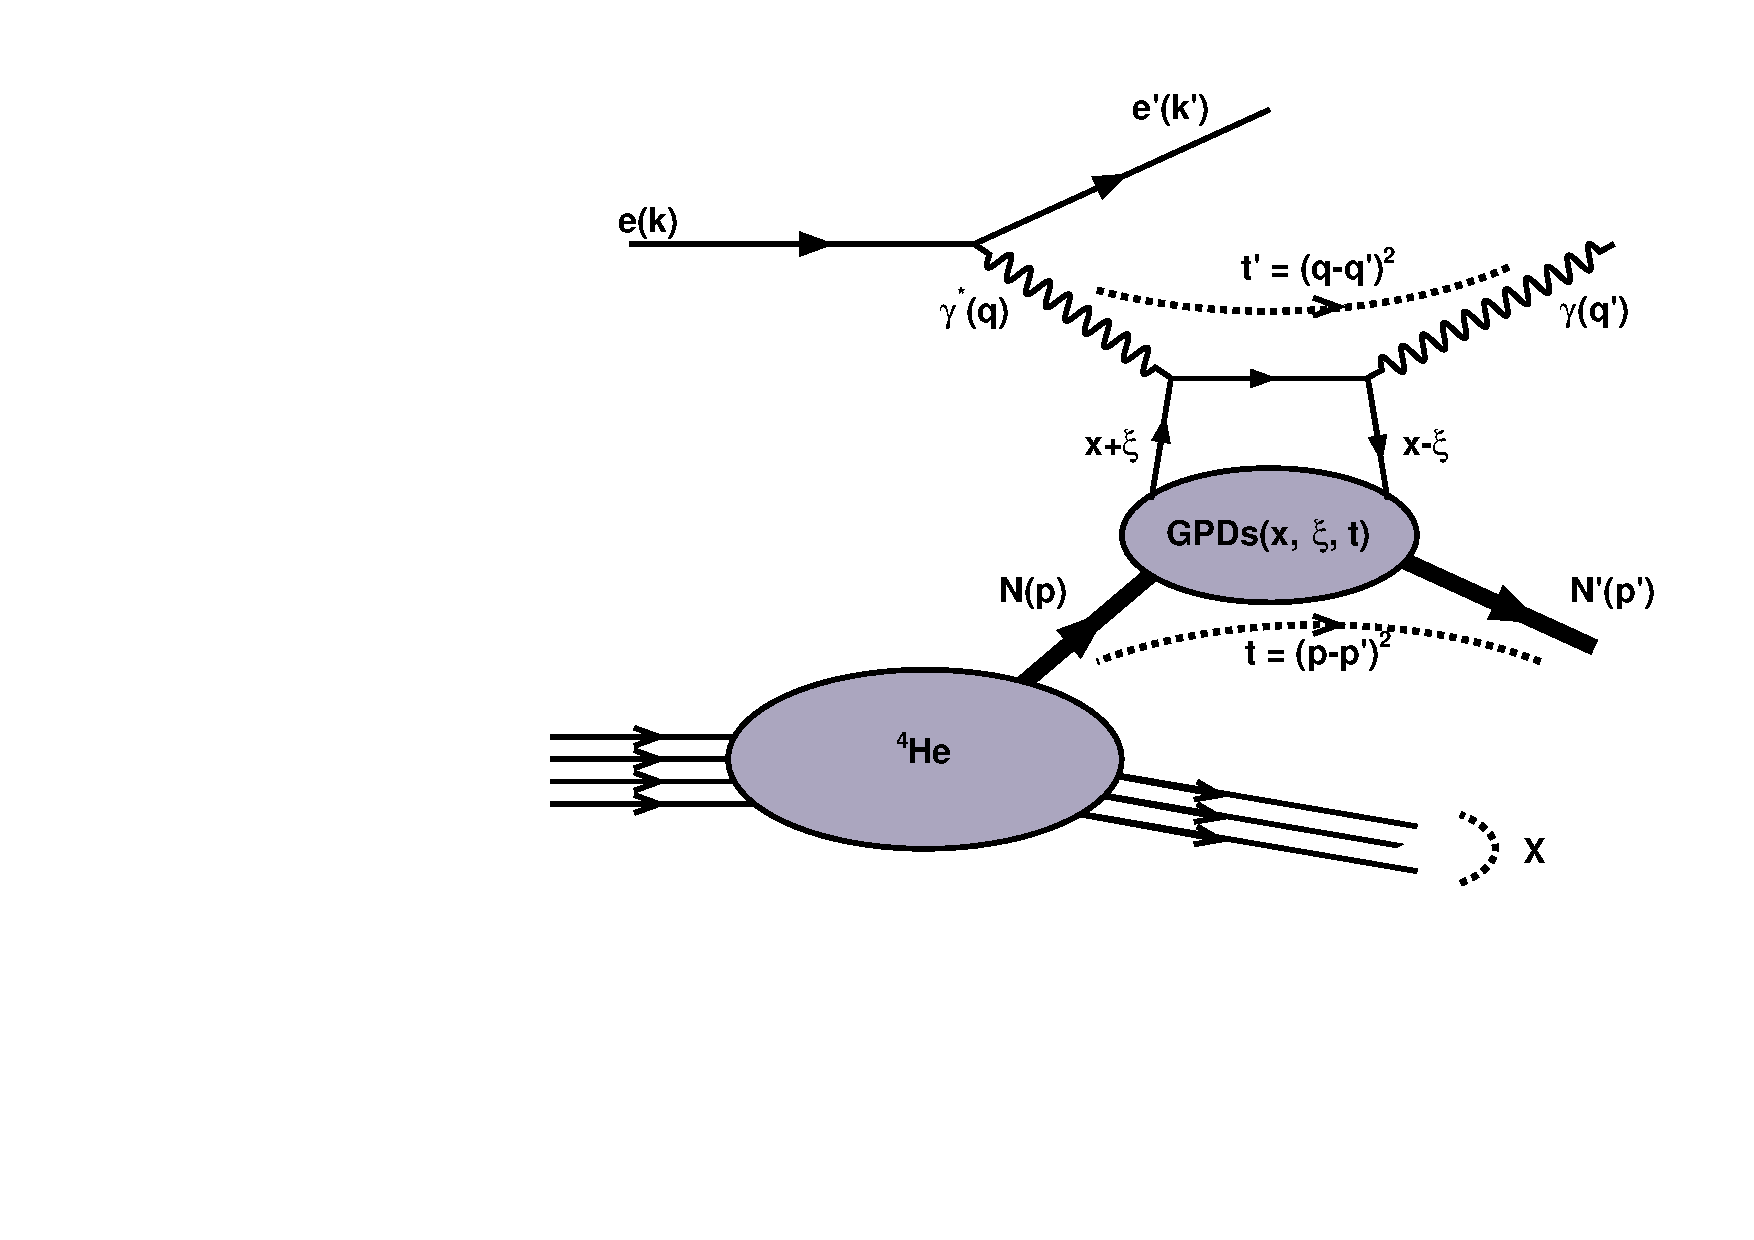
\includegraphics[height=8.0cm]{fig/handbag_incoherent.pdf}
\caption{Representation of the leading order handbag diagram of the incoherent 
DVCS process off $^4$He}
\label{fig:handbag}
\end{figure}

\section{Investigating the free proton DVCS data}

Typically, the transferred momentum squared $t$ is equal to the transferred 
momentum squared ($t'$) defined between the virtual photon and the final-state 
real photon, as shown in Figure \ref{fig:handbag}.  While defining the momentum 
transferred as $t'$ is a good way to pass the Fermi motion effect on the 
initial bound proton, $t'$ suffers from the radiative effects. In this work, we 
study the radiative effects on $t'$ using the CLAS available free proton DVCS 
data sets, E1-DVCS1 and E1-DVCS2.

Figure \ref{fig:tprime_eg6} presents the collected incoherent DVCS events from 
EG6 data binned into four bins in $t$. In order to evaluate the radiative 
effects on $t'$ we carried out a full analysis on E1-DVCS1 and E1-DVCS2 data 
sets (free proton data). The collected free proton DVCS events in the two data 
sets were binned into similar bins as our incoherent DVCS events. The results 
are presented in figure \ref{fig:tprime_e1dvcs2}.  While the EG6 incoherent 
DVCS events show a relatively more smeared $\frac{t'-t}{t}$ distributions than 
the free proton data sets, the free proton sets show a significant shifts 
specially at low $t$ values.  

\begin{figure}[h!]
\centering
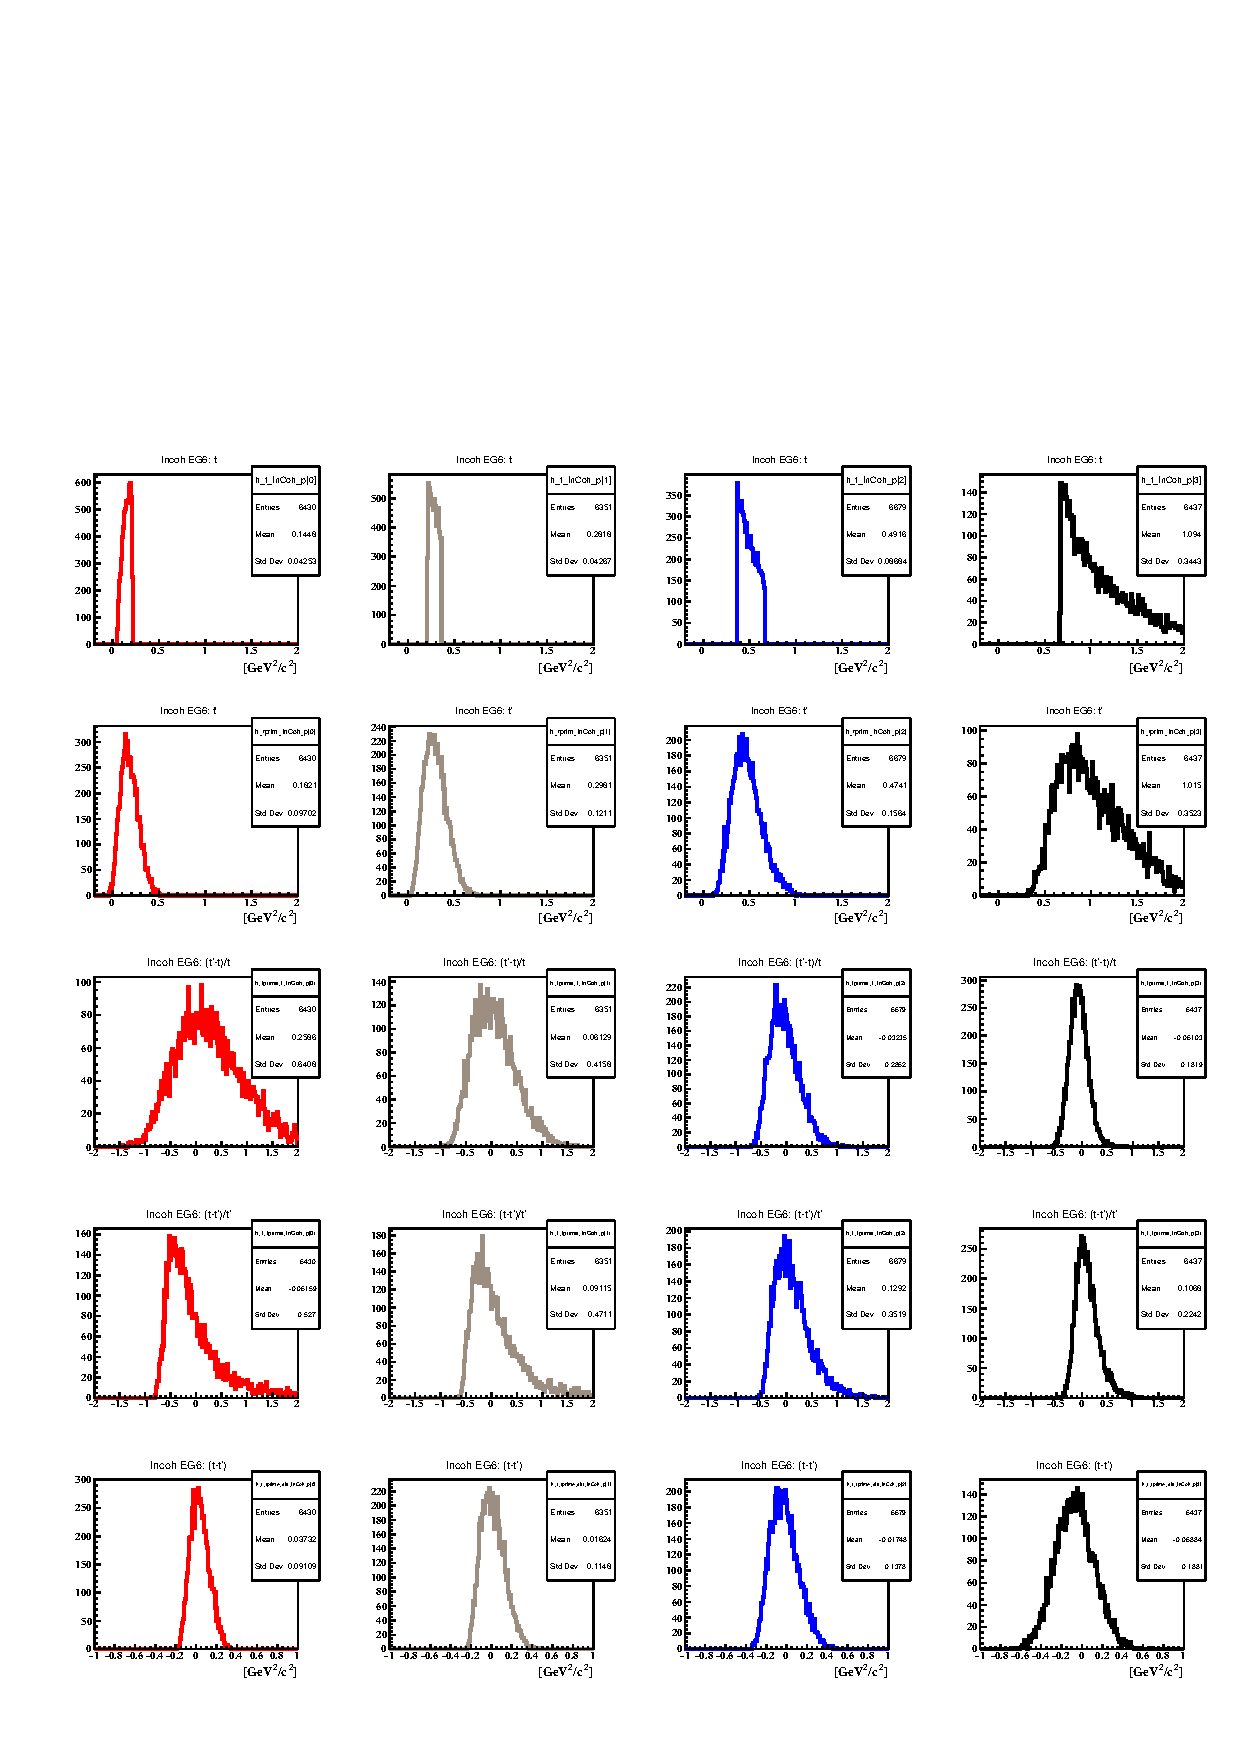
\includegraphics[height=19.0cm]{fig/t_tprime_Incoh.pdf}
\caption{The EG6 incoherent DVCS sample. The first row presents the four bins 
in $t$. The second row shows the distribution of $t'$ for the DVCS events in 
each bin in $t$ in the first row plots. The third row shows $\frac{t'-t}{t}$.  
The 4$^{th}$ shows $\frac{t-t'}{t'}$, and the 5$^{th}$ shows $t-t'$.}
\label{fig:tprime_eg6}
\end{figure}

%\begin{figure}[h!]
%\centering
%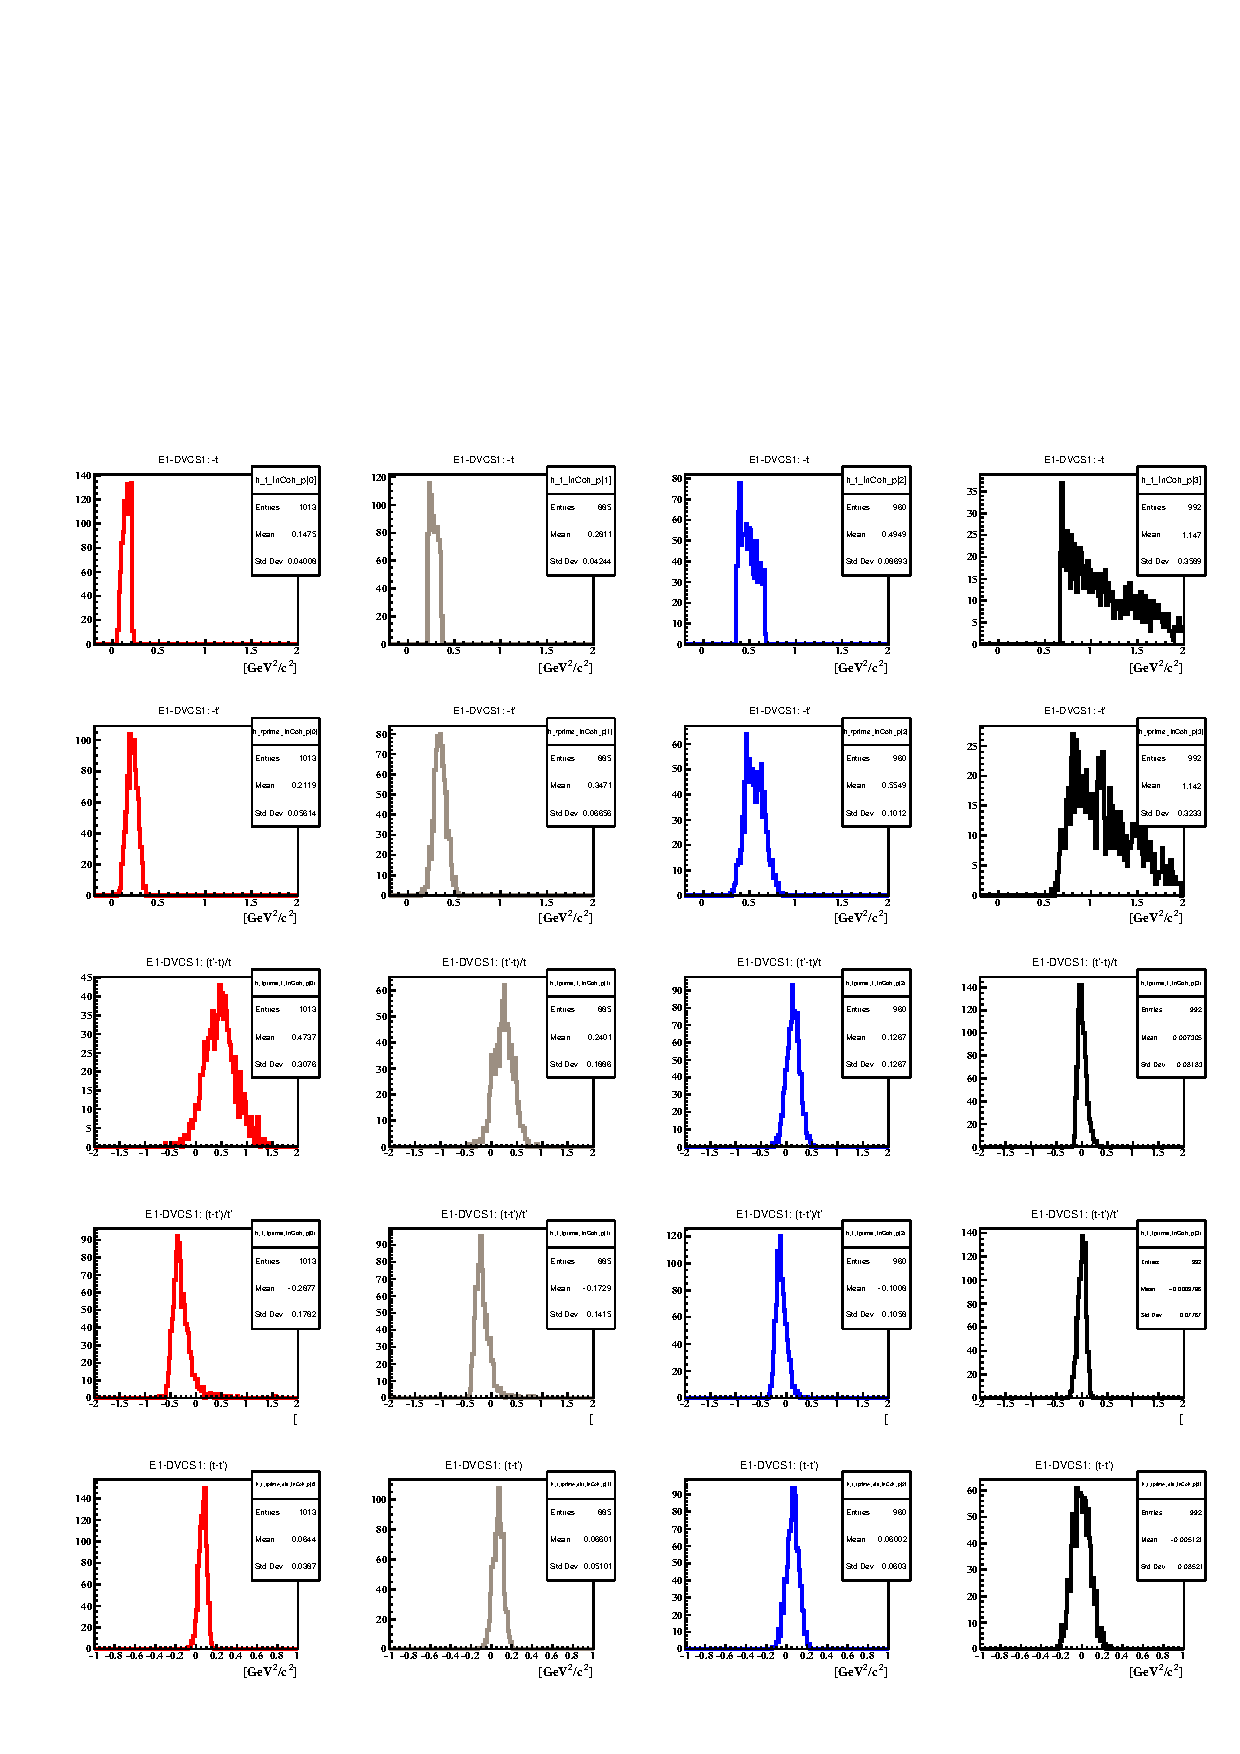
\includegraphics[height=19.0cm]{fig/E1-dvcs1-t_tprime_Incoh.pdf}
%\caption{The E1-DVCS1 free proton DVCS sample. See the caption of figure 
%\ref{fig:tprime_eg6} for plots description.}
%\label{fig:tprime_e1dvcs1}
%\end{figure}

\begin{figure}[h!]
\centering
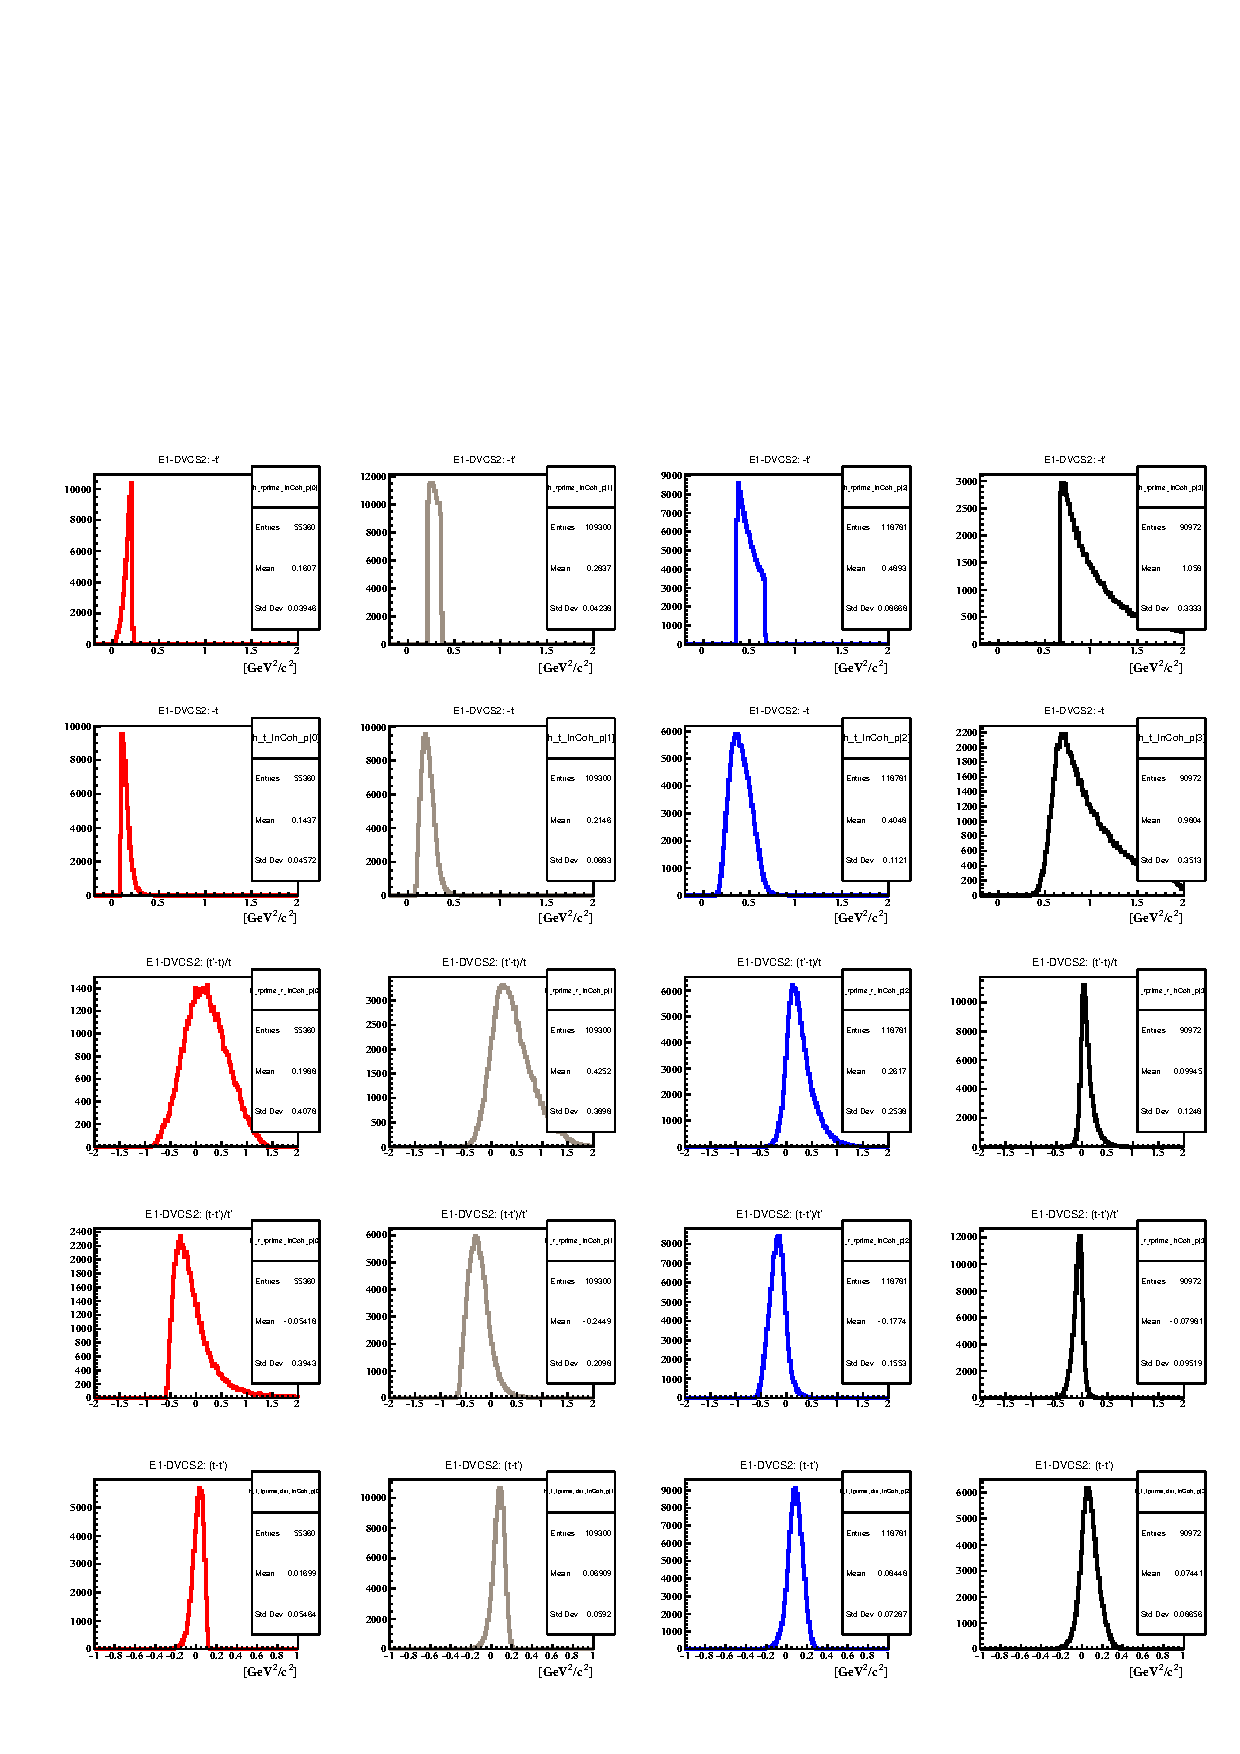
\includegraphics[height=19.0cm]{fig/before_corrections_E1-dvcs2-t_tprime_Incoh.pdf}
\caption{The E1-DVCS2 free proton DVCS sample BEFORE correcting $t'$. See the 
caption of figure \ref{fig:tprime_eg6} for plots description.}
\label{fig:tprime_e1dvcs2}
\end{figure}


\section{$t'$ correction}
One can see from the free proton DVCS sample, figure \ref{fig:tprime_e1dvcs2}, 
that $t'$ is slightly shifted compared to $t$, which is considered as the true 
value in the free proton case. This shift in $t'$ is mainly induced by the 
radiative effects on the leptons. Before considering $t'$ in the incoherent EG6 
analysis, $t'$ has to be corrected and the reconstructed free proton 
asymmetries have to be verified in order to estimate the associated systematic 
uncertainties. Figure \ref{fig:corrections_tprime_e1dvcs2} presents the 
distributions of $t-t'$ as a function of $t'$ for the free proton DVCS sample 
from E1-DVCS2 data before and after correcting $t'$. In figure 
\ref{fig:after_tprime_e1dvcs2}, the distributions of figure 
\ref{fig:tprime_e1dvcs2} are shown after the $t'$ corrections.

\begin{figure}[h!]
\centering
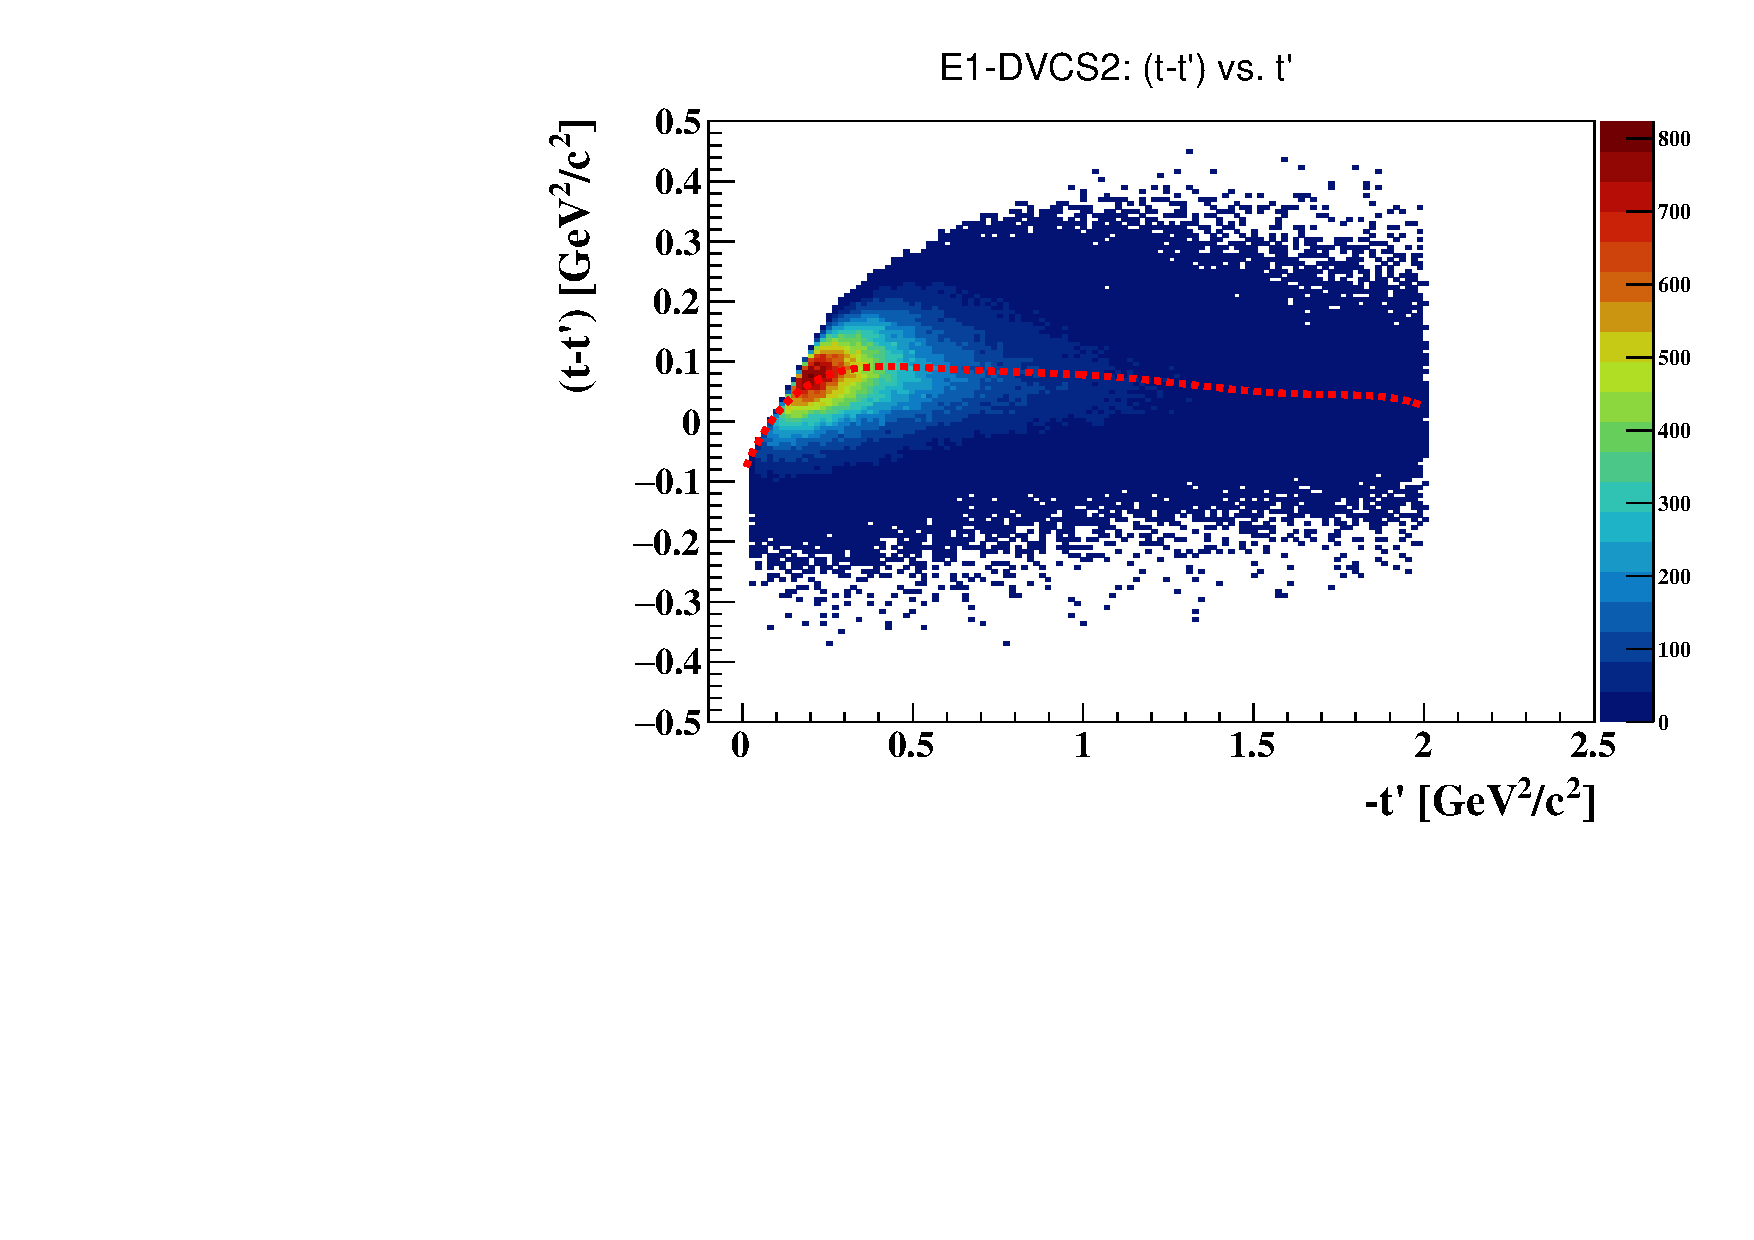
\includegraphics[height=10.0cm]{fig/before_corrections_tprimet_t_InCoh.pdf}
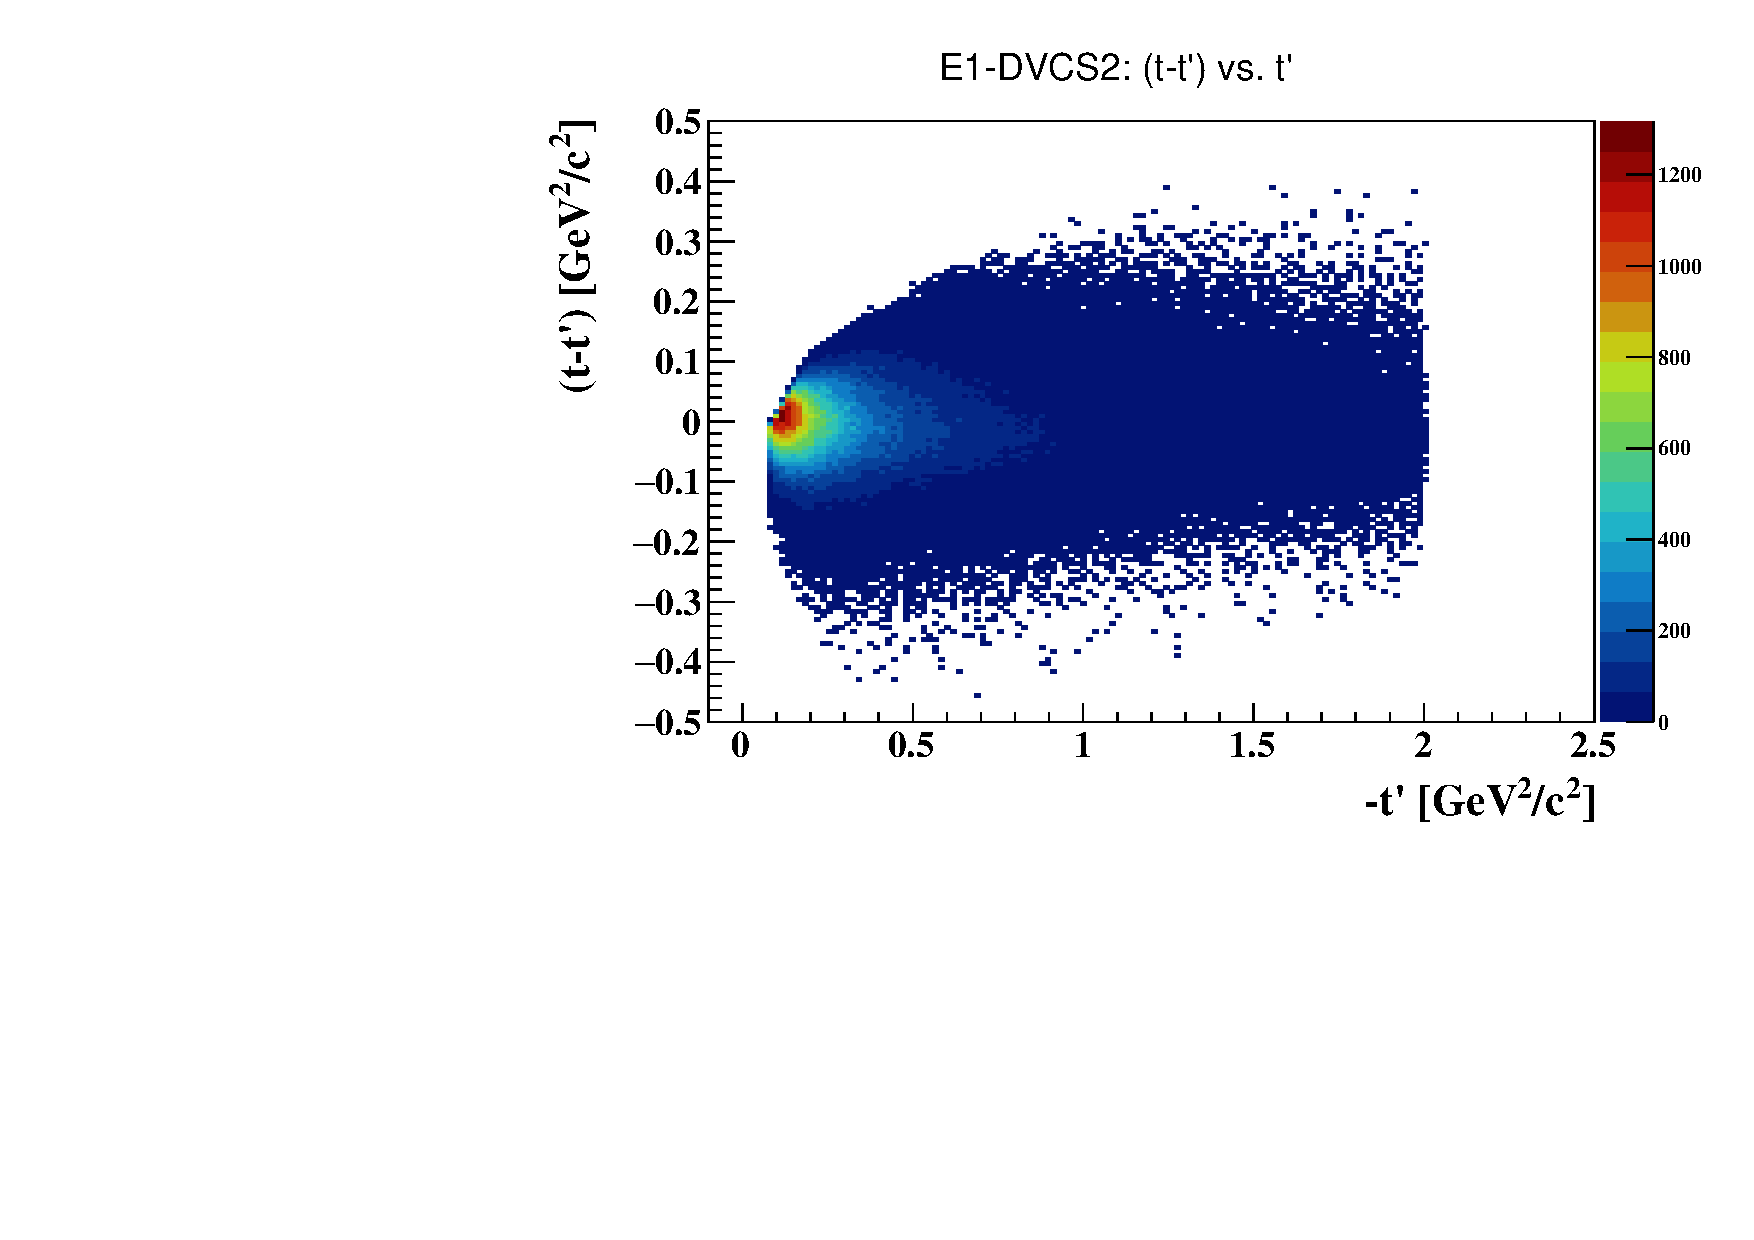
\includegraphics[height=10.0cm]{fig/after_corrections_tprimet_t_InCoh.pdf}
\caption{On top: $t-t'$ as a function of $t'$ for the E1-DVCS2 free proton DVCS 
sample BEFORE correcting $t'$. The red line is the extracted correction for 
$t'$. On bottom: $t-t'$ as a function of $t'$ after correcting $t'$.}
\label{fig:corrections_tprime_e1dvcs2}
\end{figure}

\begin{figure}[h!]
\centering
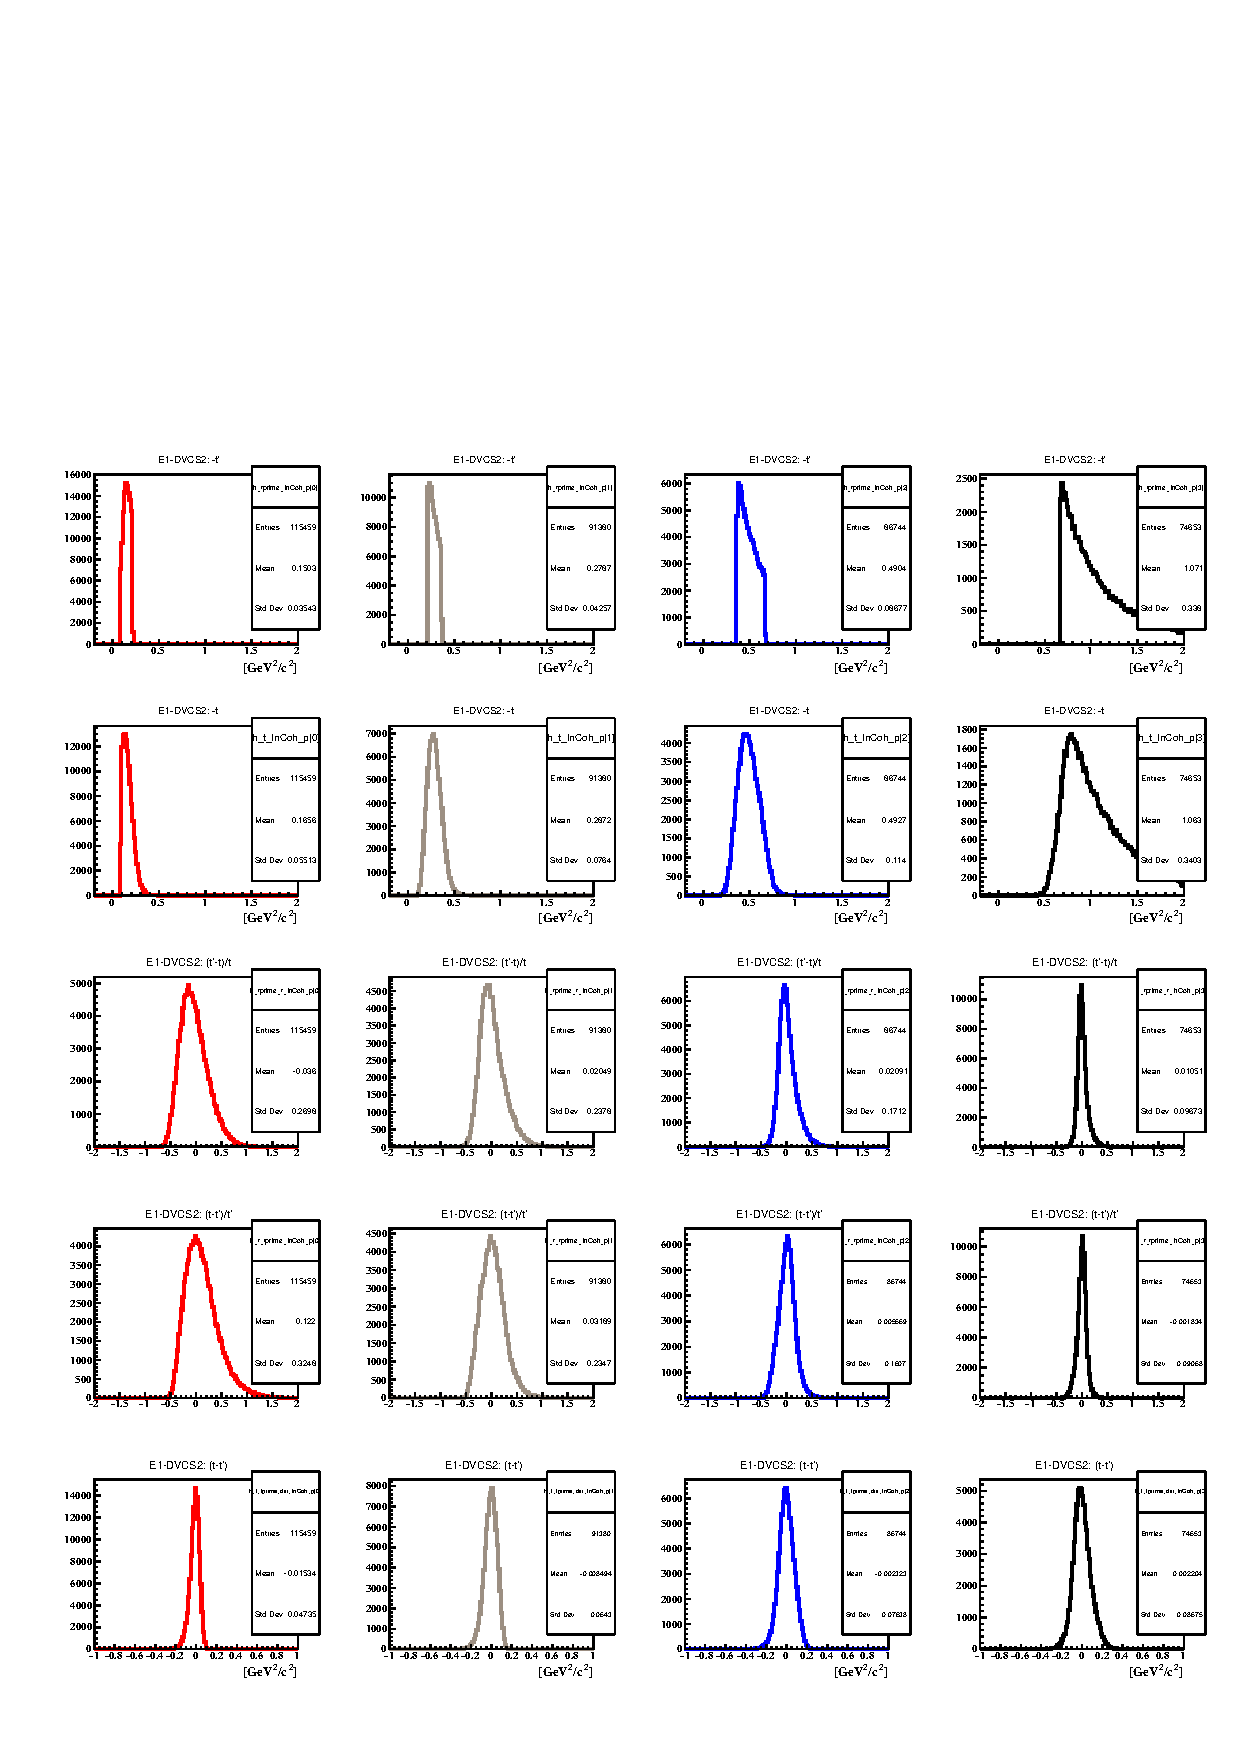
\includegraphics[height=19.0cm]{fig/after_corrections_E1-dvcs2-t_tprime_Incoh.pdf}
\caption{The E1-DVCS2 free proton DVCS sample AFTER correcting $t'$. See the 
caption of figure \ref{fig:tprime_eg6} for plots description.}
\label{fig:after_tprime_e1dvcs2}
\end{figure}





\section{Comparing the $t$ and the corrected $t'$ asymmetries in the E1-DVCS2 
data set}
Here we compare the E1-DVCS2 free proton DVCS beam-spin asymmetries using $t$ 
and the corrected $t'$ to estimate the associated systematic uncertainties.  
Figure \ref{t_tprime_ALU_phi} presents the reconstructed $A_{LU}$ as a function 
of $\phi$ in the same binning as the incoherent EG6 DVCS channel. The binning 
in $t$ and the corrected $t'$ are the same. Figure \ref{fig:t_tprime_ALU_90} 
presents the $A_{LU}$ at $\phi = 90^{\circ}$ from the fits in figure 
\ref{fig:t_tprime_ALU_phi}, as a function of $t$ and the corrected $t'$ showing 
the estimated systematic uncertainties. No induced systematic uncertainties are 
observed on the $Q^{2}$ and $x_B$, while some appear on $t$, which will be 
added to the EG6 incoherent asymmetries. 


\begin{figure}[h!]
\centering
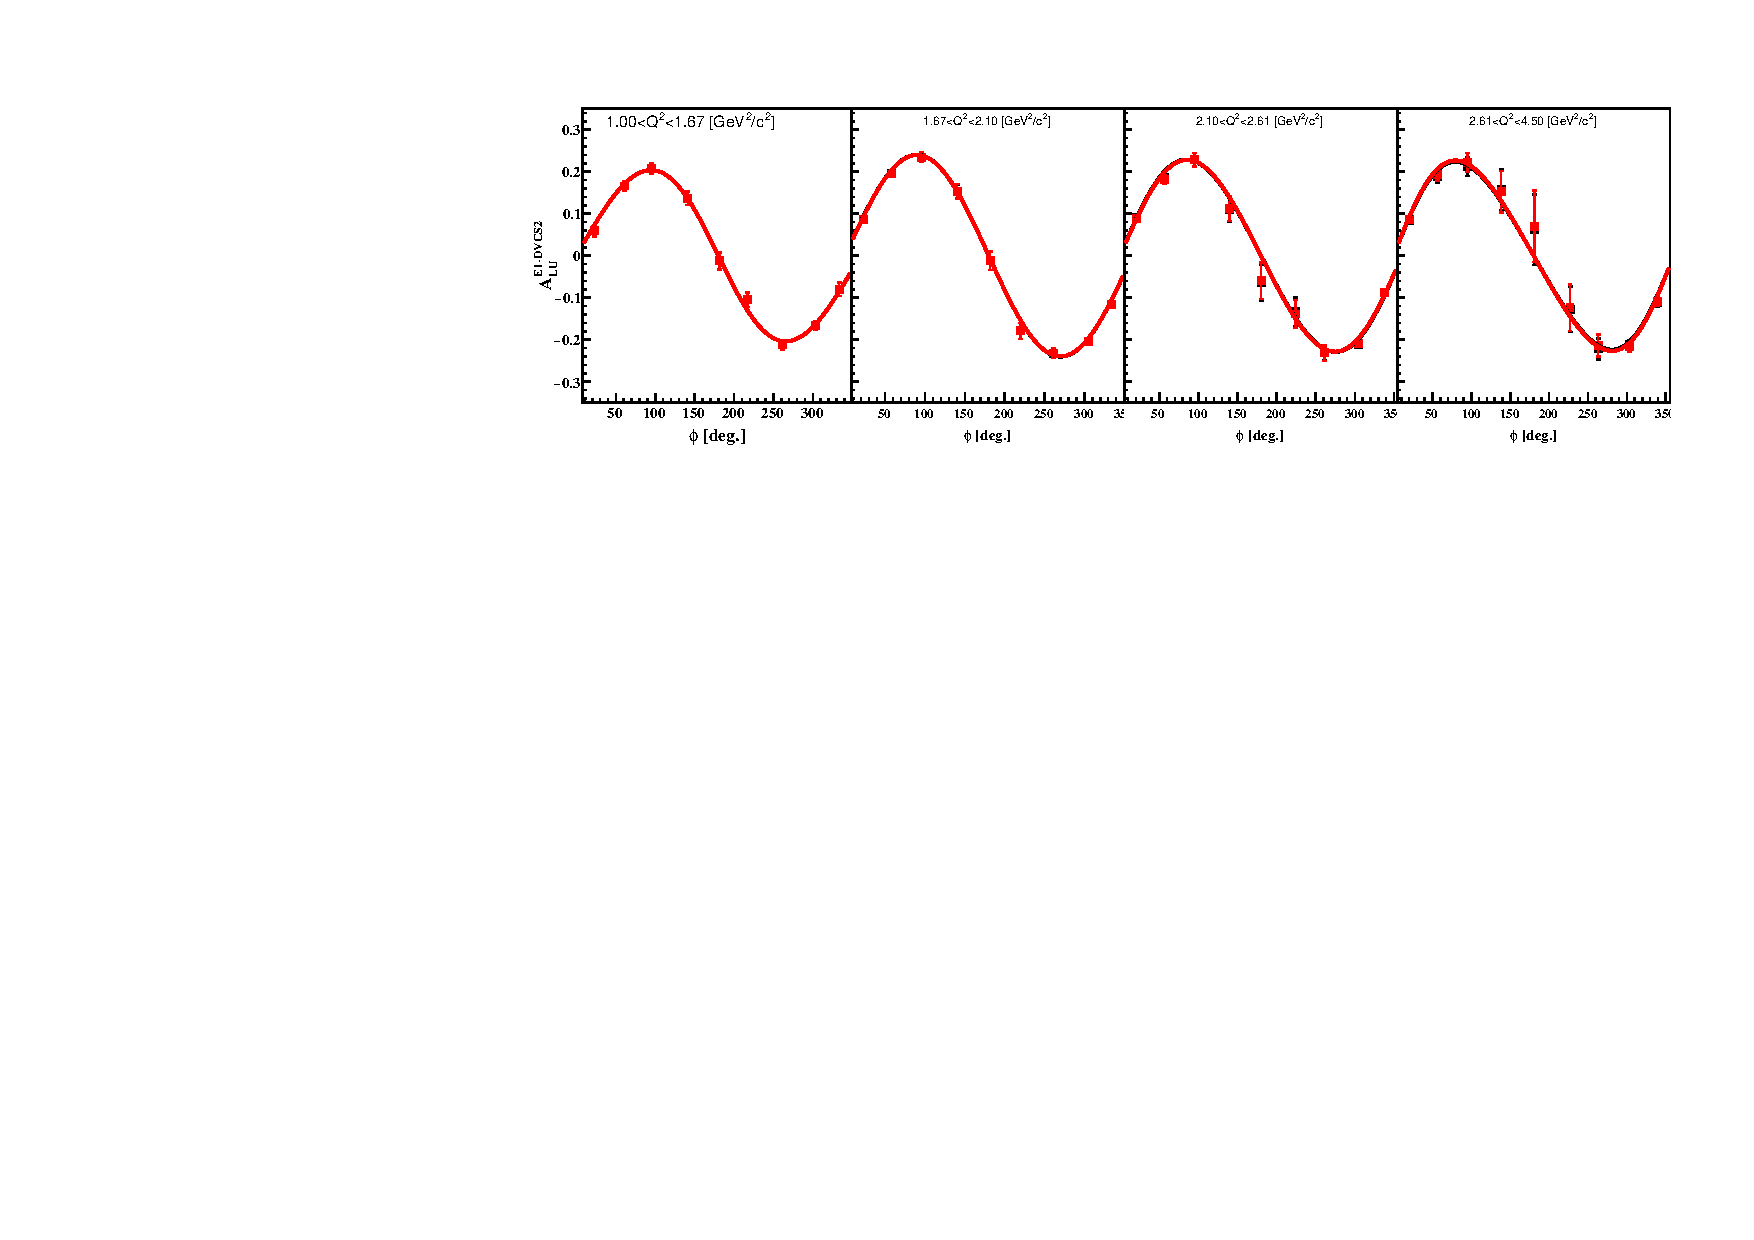
\includegraphics[height=6.0cm]{fig/E1DVCS2-ALU_phi_p_Q2.pdf}
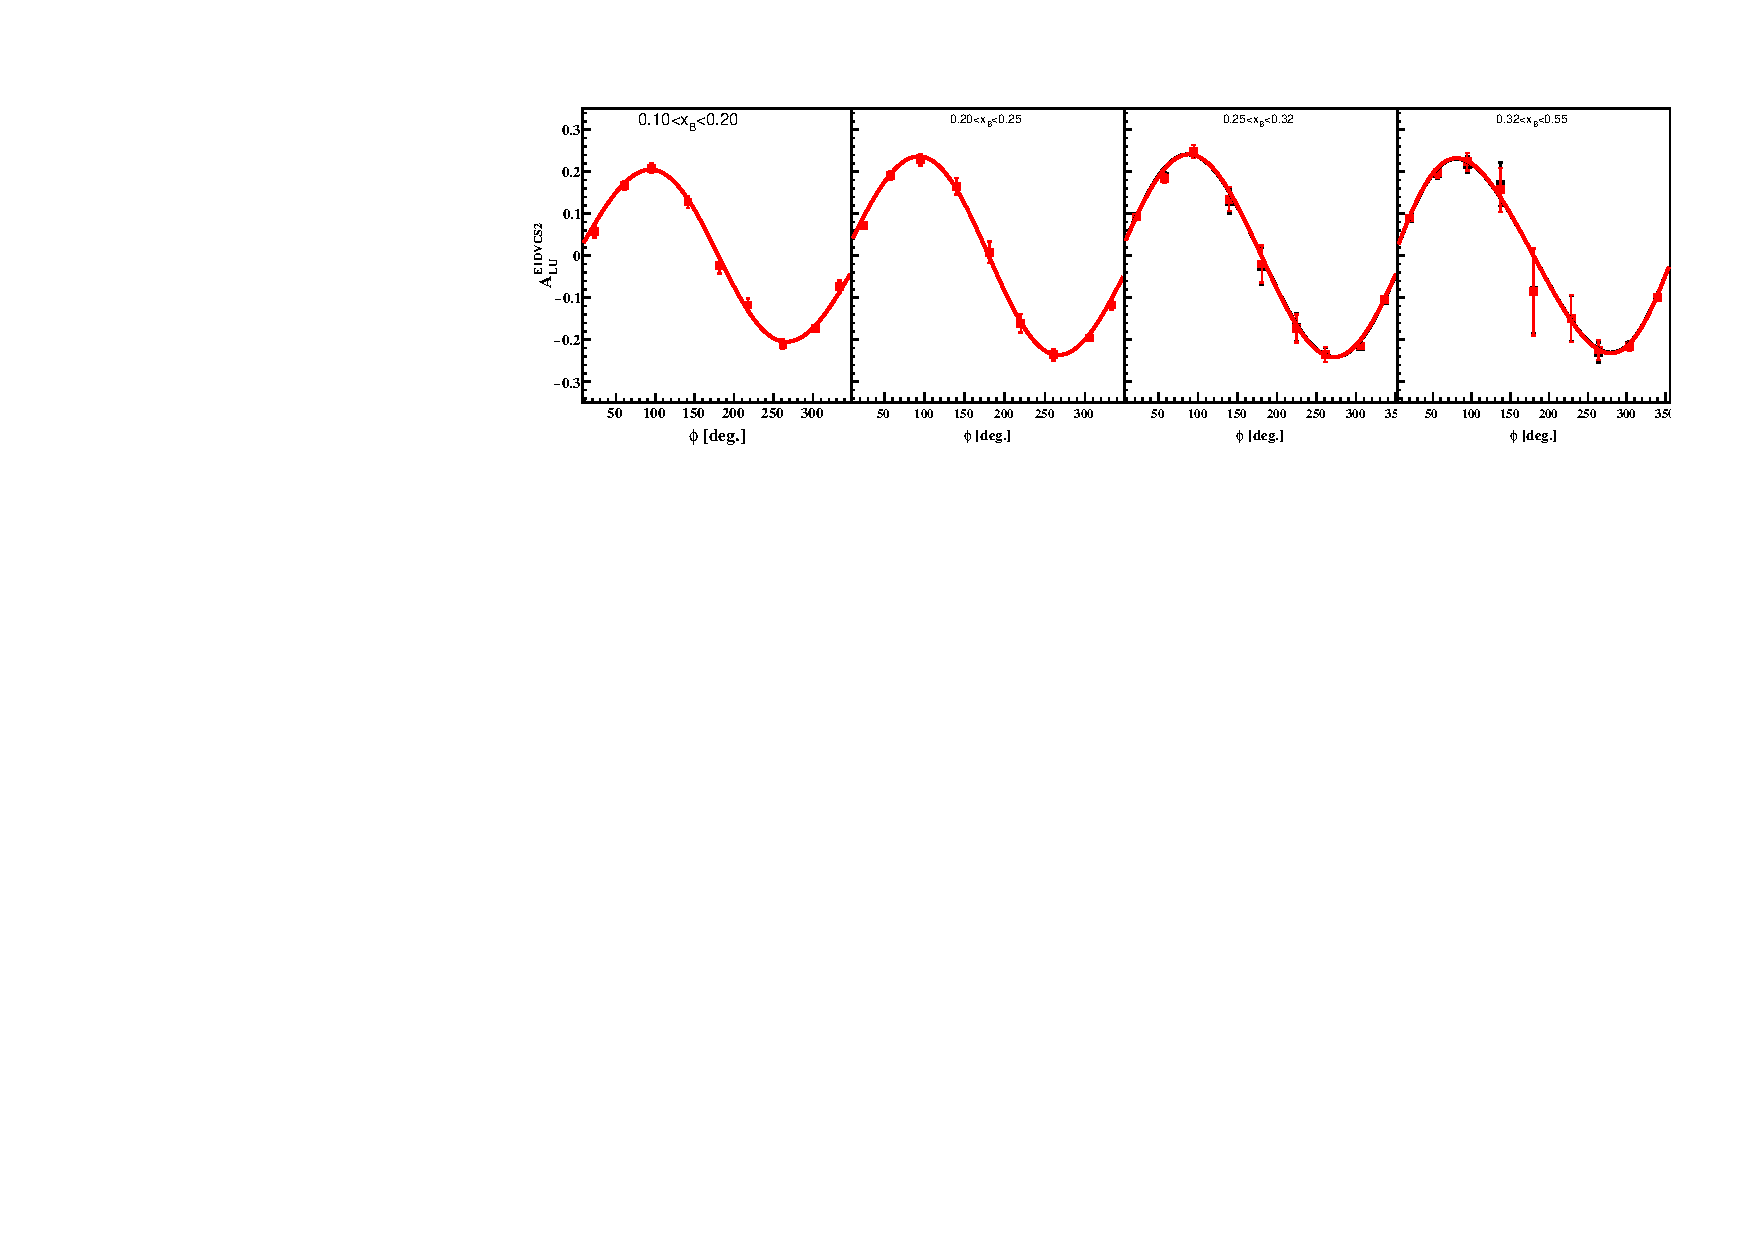
\includegraphics[height=6.0cm]{fig/E1DVCS2-ALU_phi_p_x.pdf}
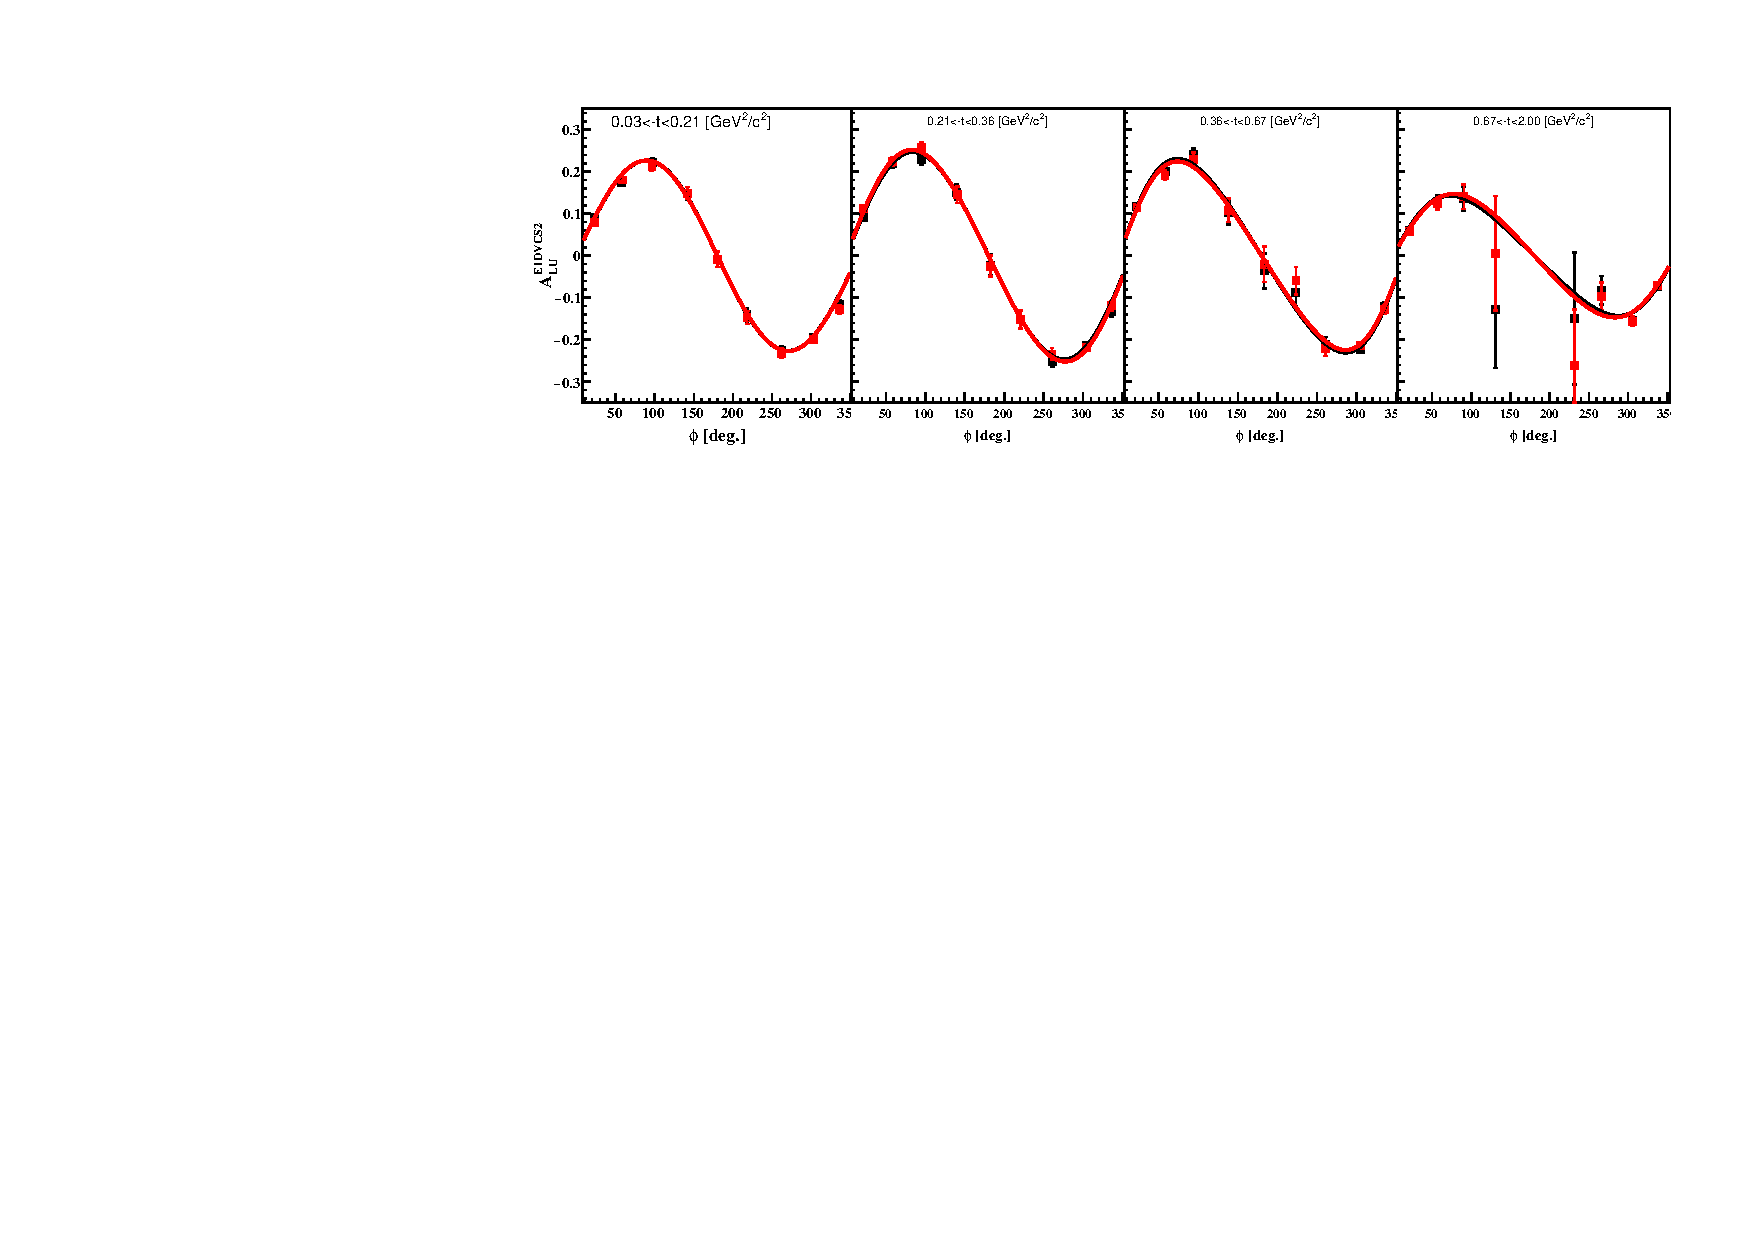
\includegraphics[height=6.0cm]{fig/E1DVCS2-ALU_phi_p_t.pdf}
\caption{The reconstructed $A_{LU}$ as a function of $\phi$ for the collected 
E1-DVCS2 free proton DVCS sample using $t$ in black points and using the 
corrected $t'$ in red points. The lines represent fits in the form of 
$\frac{\alpha sin(\phi)}{1+\beta cos(\phi)}$ for the two sets of analysis.}
\label{fig:t_tprime_ALU_phi}
\end{figure}

\begin{figure}[h!]
\centering
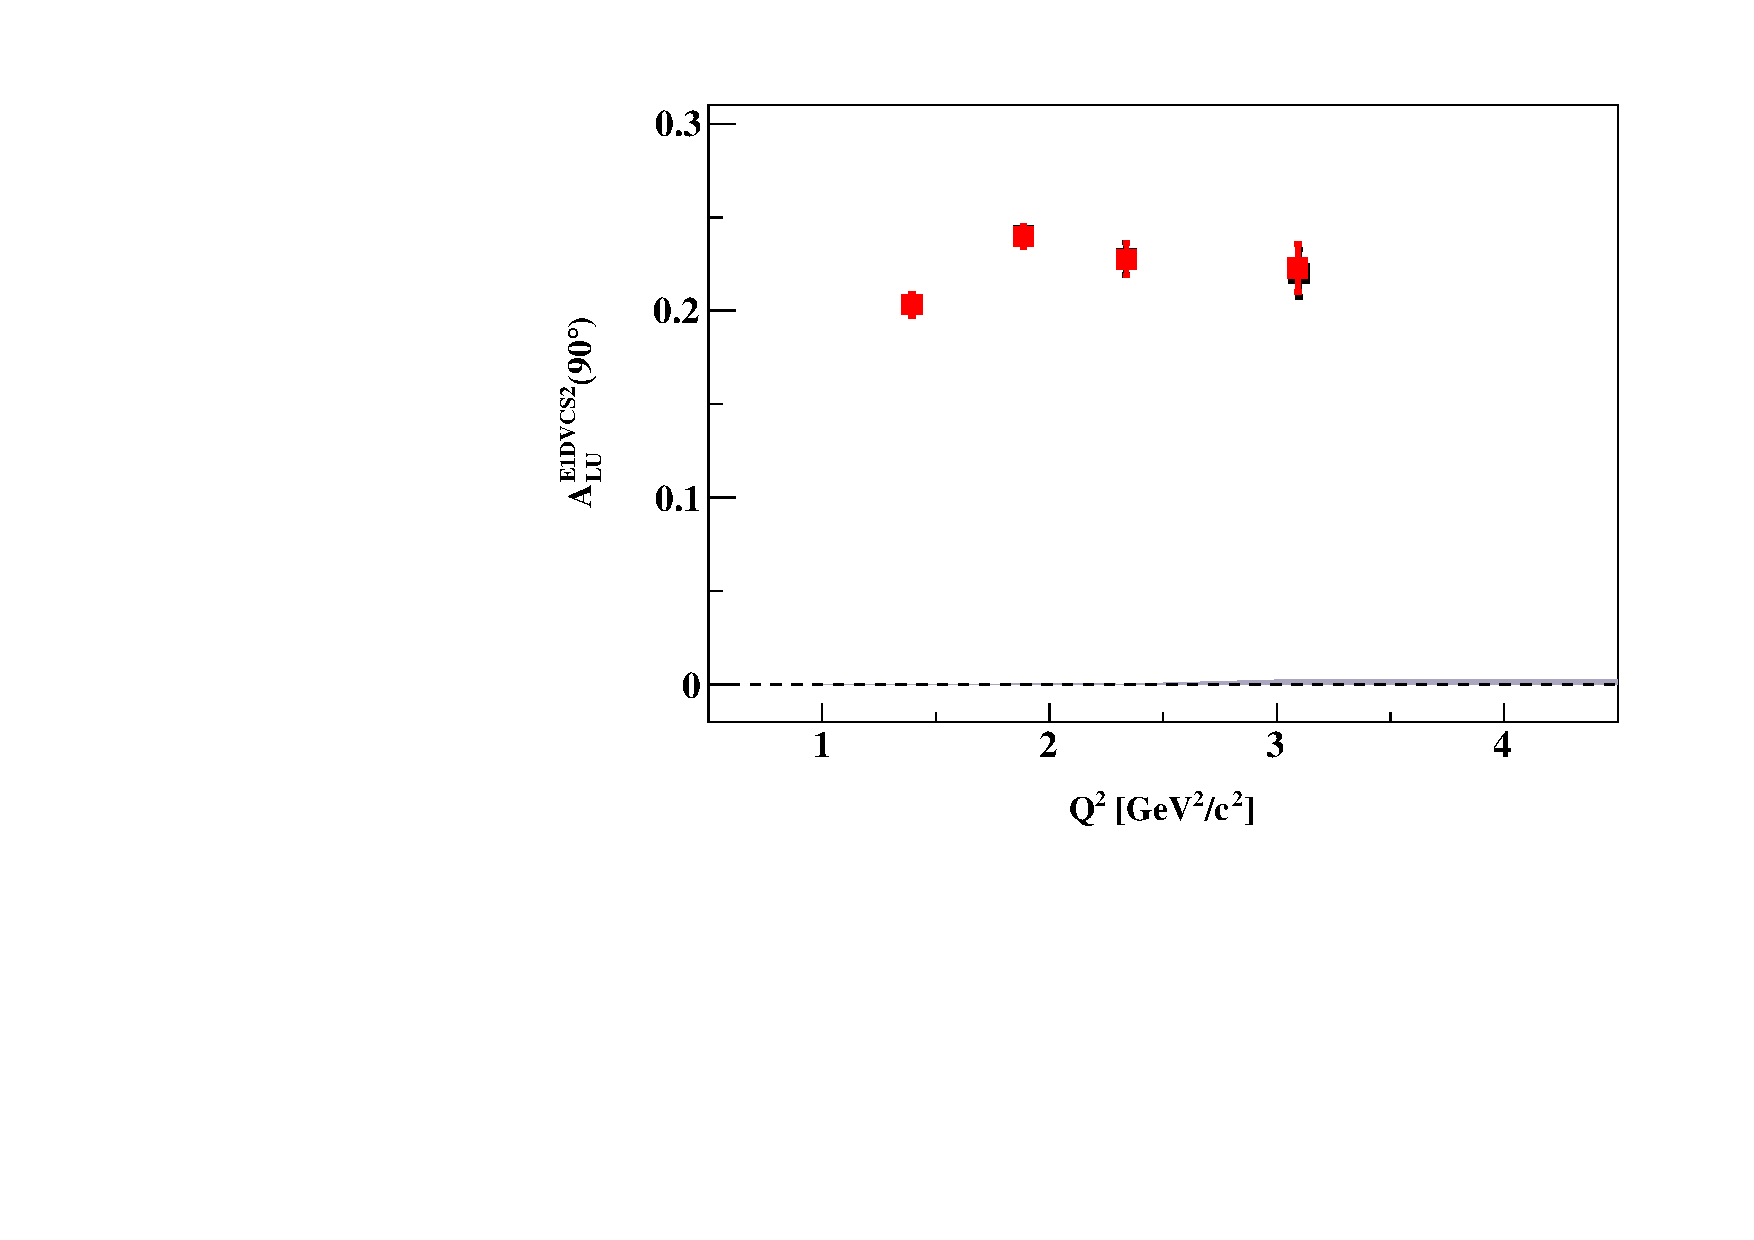
\includegraphics[height=7.0cm]{fig/E1DVCS2-ALU_90_p_vs_Q2_shortscenrario.pdf}
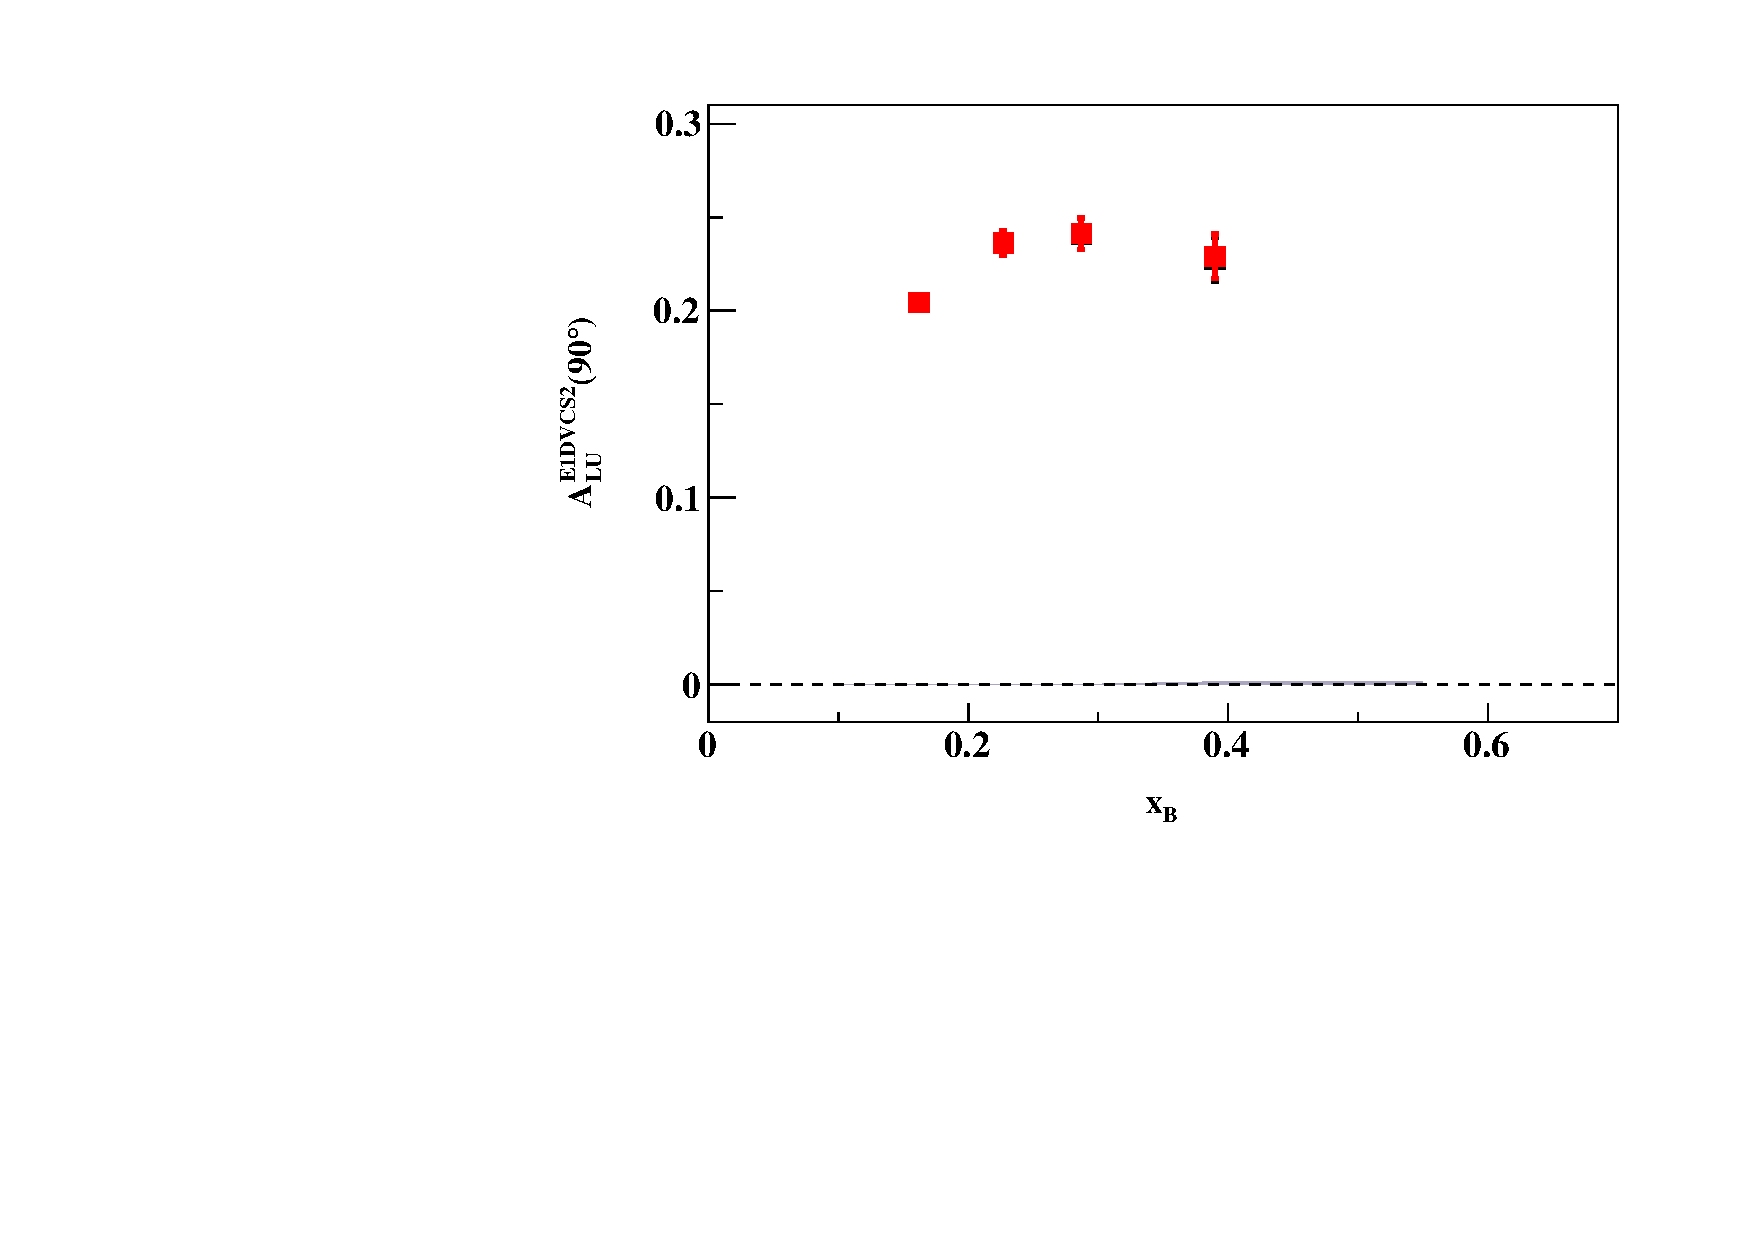
\includegraphics[height=7.0cm]{fig/E1DVCS2-ALU_90_p_vs_x_shortscenrario.pdf}
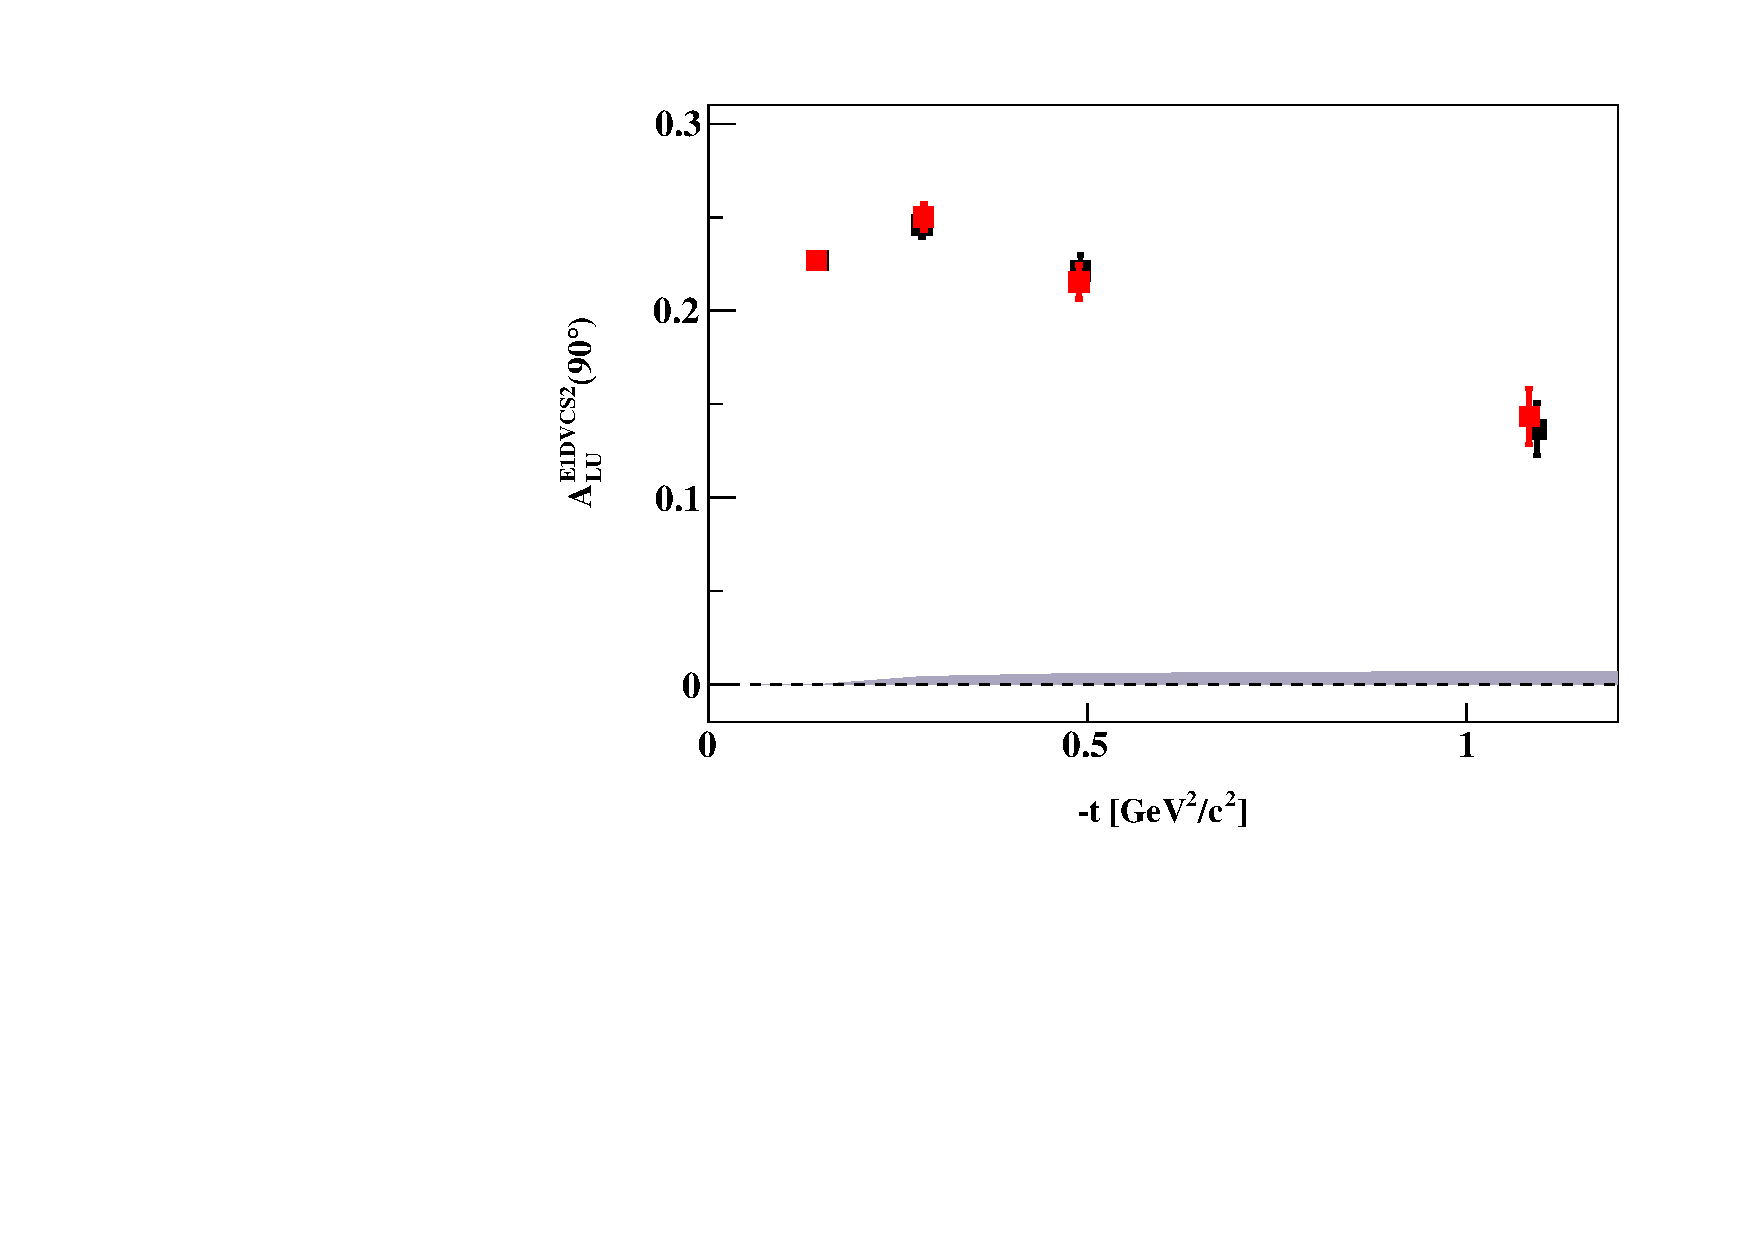
\includegraphics[height=7.0cm]{fig/E1DVCS2-ALU_90_p_vs_t_shortscenrario.pdf}
\caption{$A_{LU}$ at $\phi = 90^{\circ}$ from the fits in figure 
\ref{fig:t_tprime_ALU_phi} as a function of $t$ in black points and as a 
function of the corrected $t'$ in red points.}
\label{fig:t_tprime_ALU_90}
\end{figure}


\section{EG6 Incoherent DVCS channel}
Here we apply the $t'$ corrections that were extracted from the free proton 
asymmetries  to the EG6 incoherent DVCS channel. Then, the asymmetries using 
$t$ are compared to the ones reconstructed using the corrected $t'$. The 
results are presented in figures \ref{fig:alu} and \ref{fig:alu90}.

\begin{figure}[tb]
   \centering
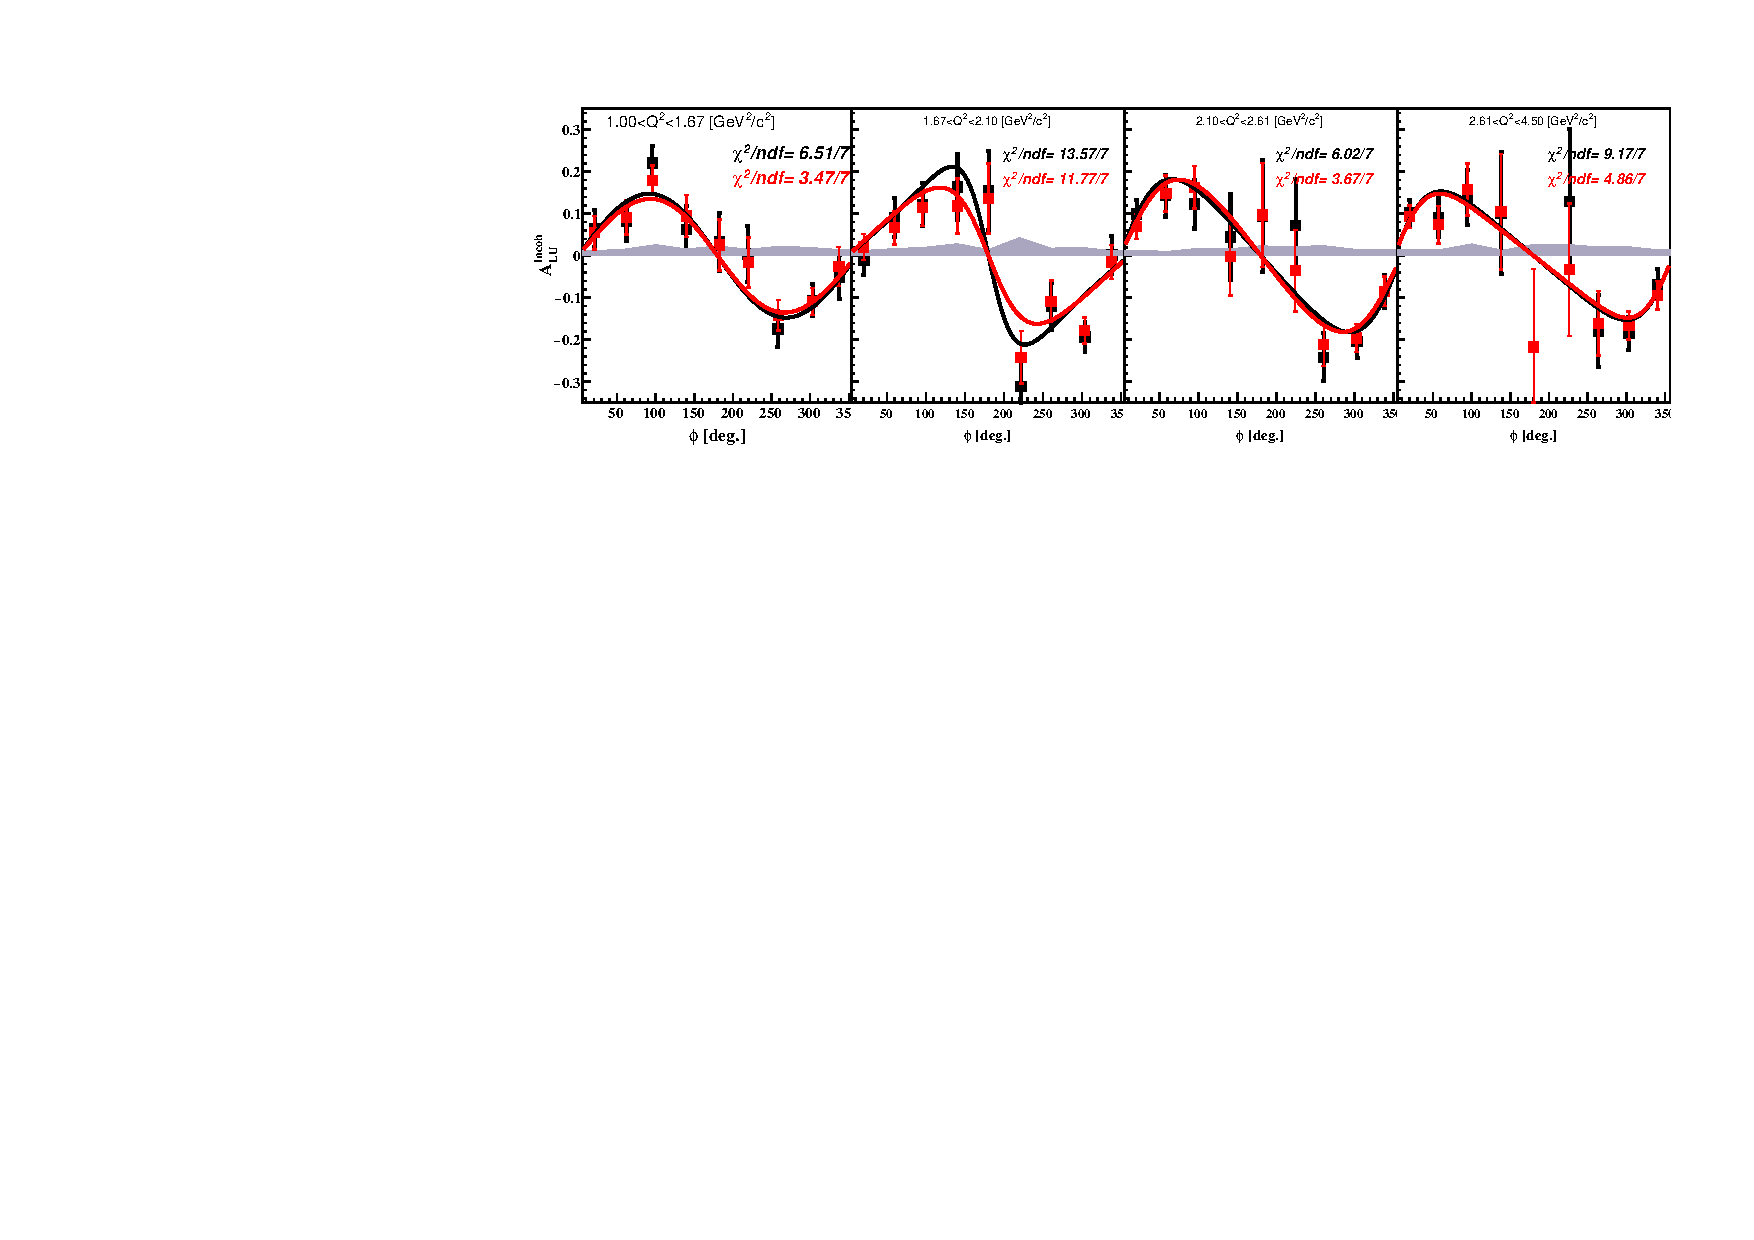
\includegraphics[width=15cm]{fig/ALU_phi_p_Q2.pdf}
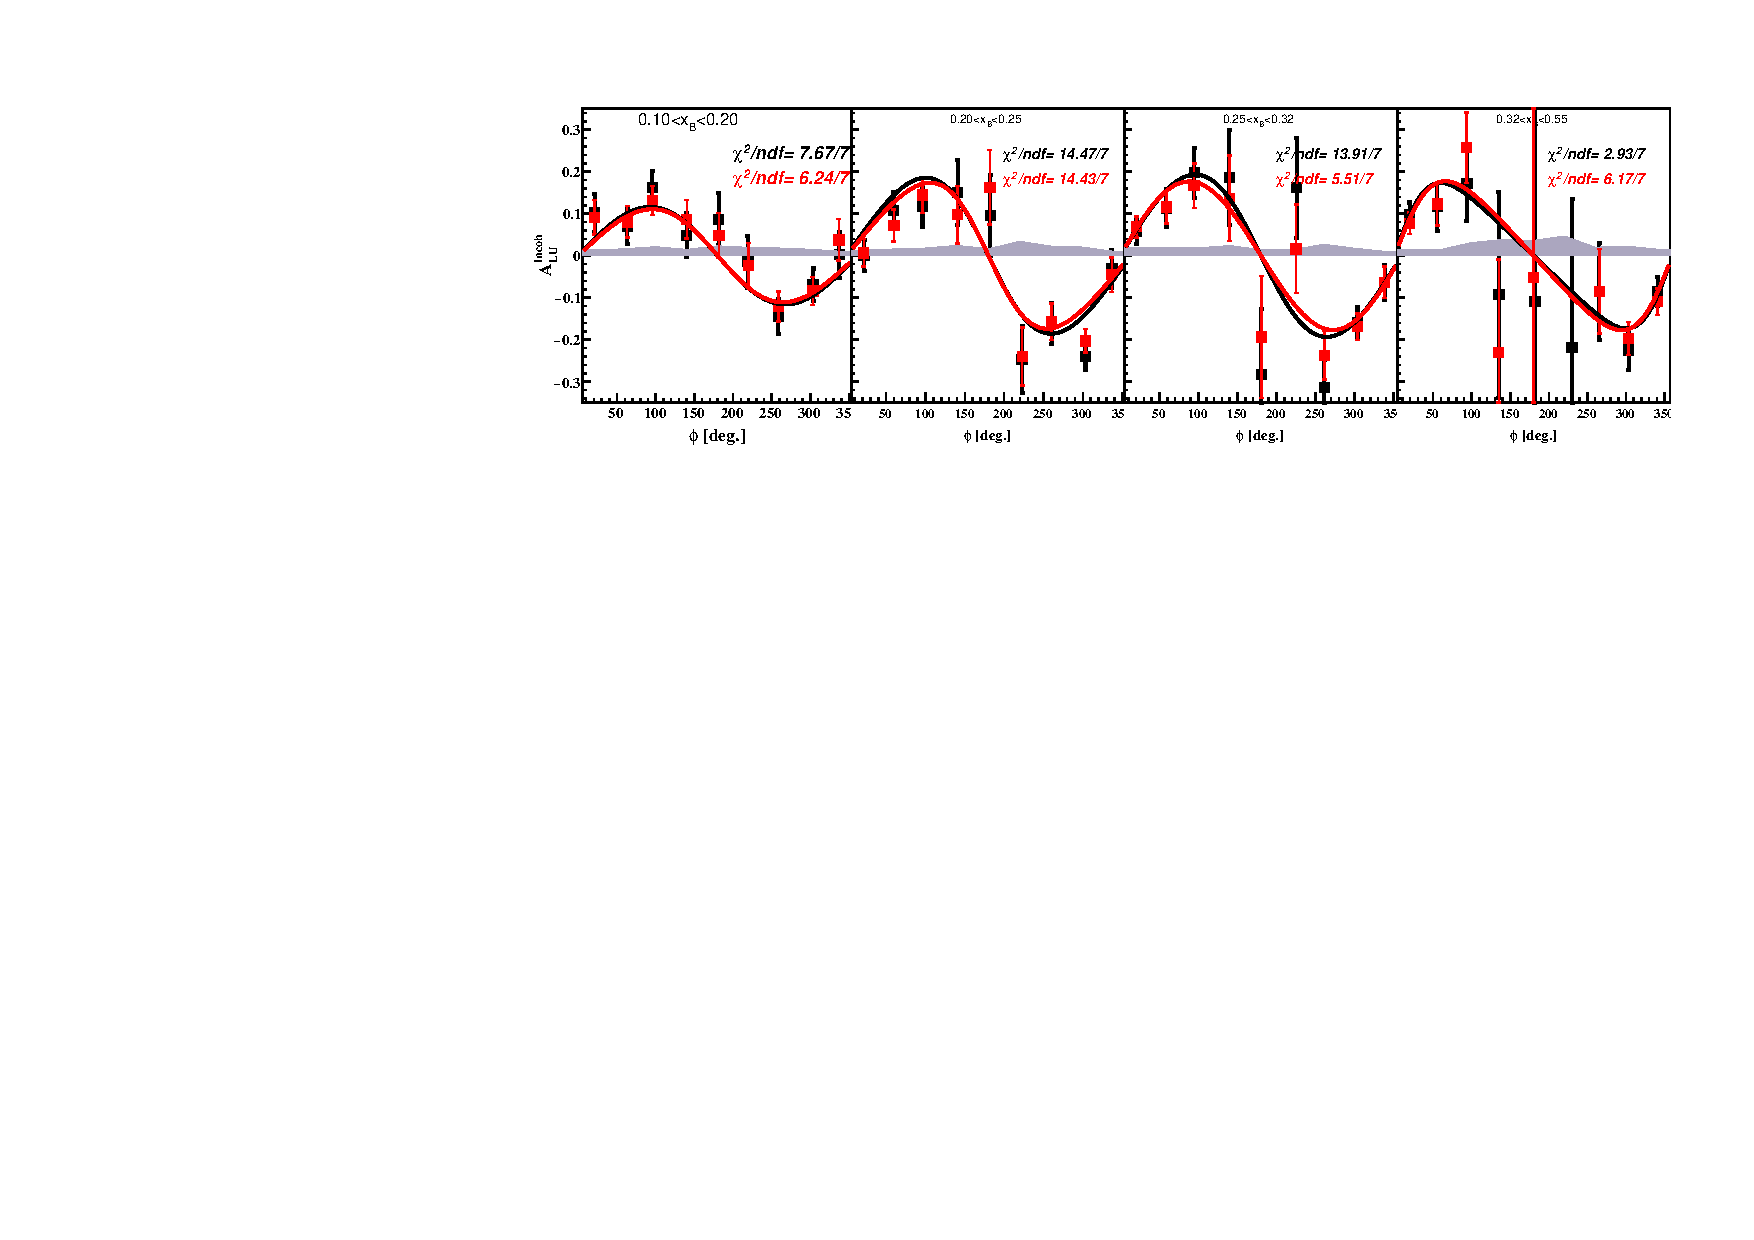
\includegraphics[width=15cm]{fig/ALU_phi_p_x.pdf}
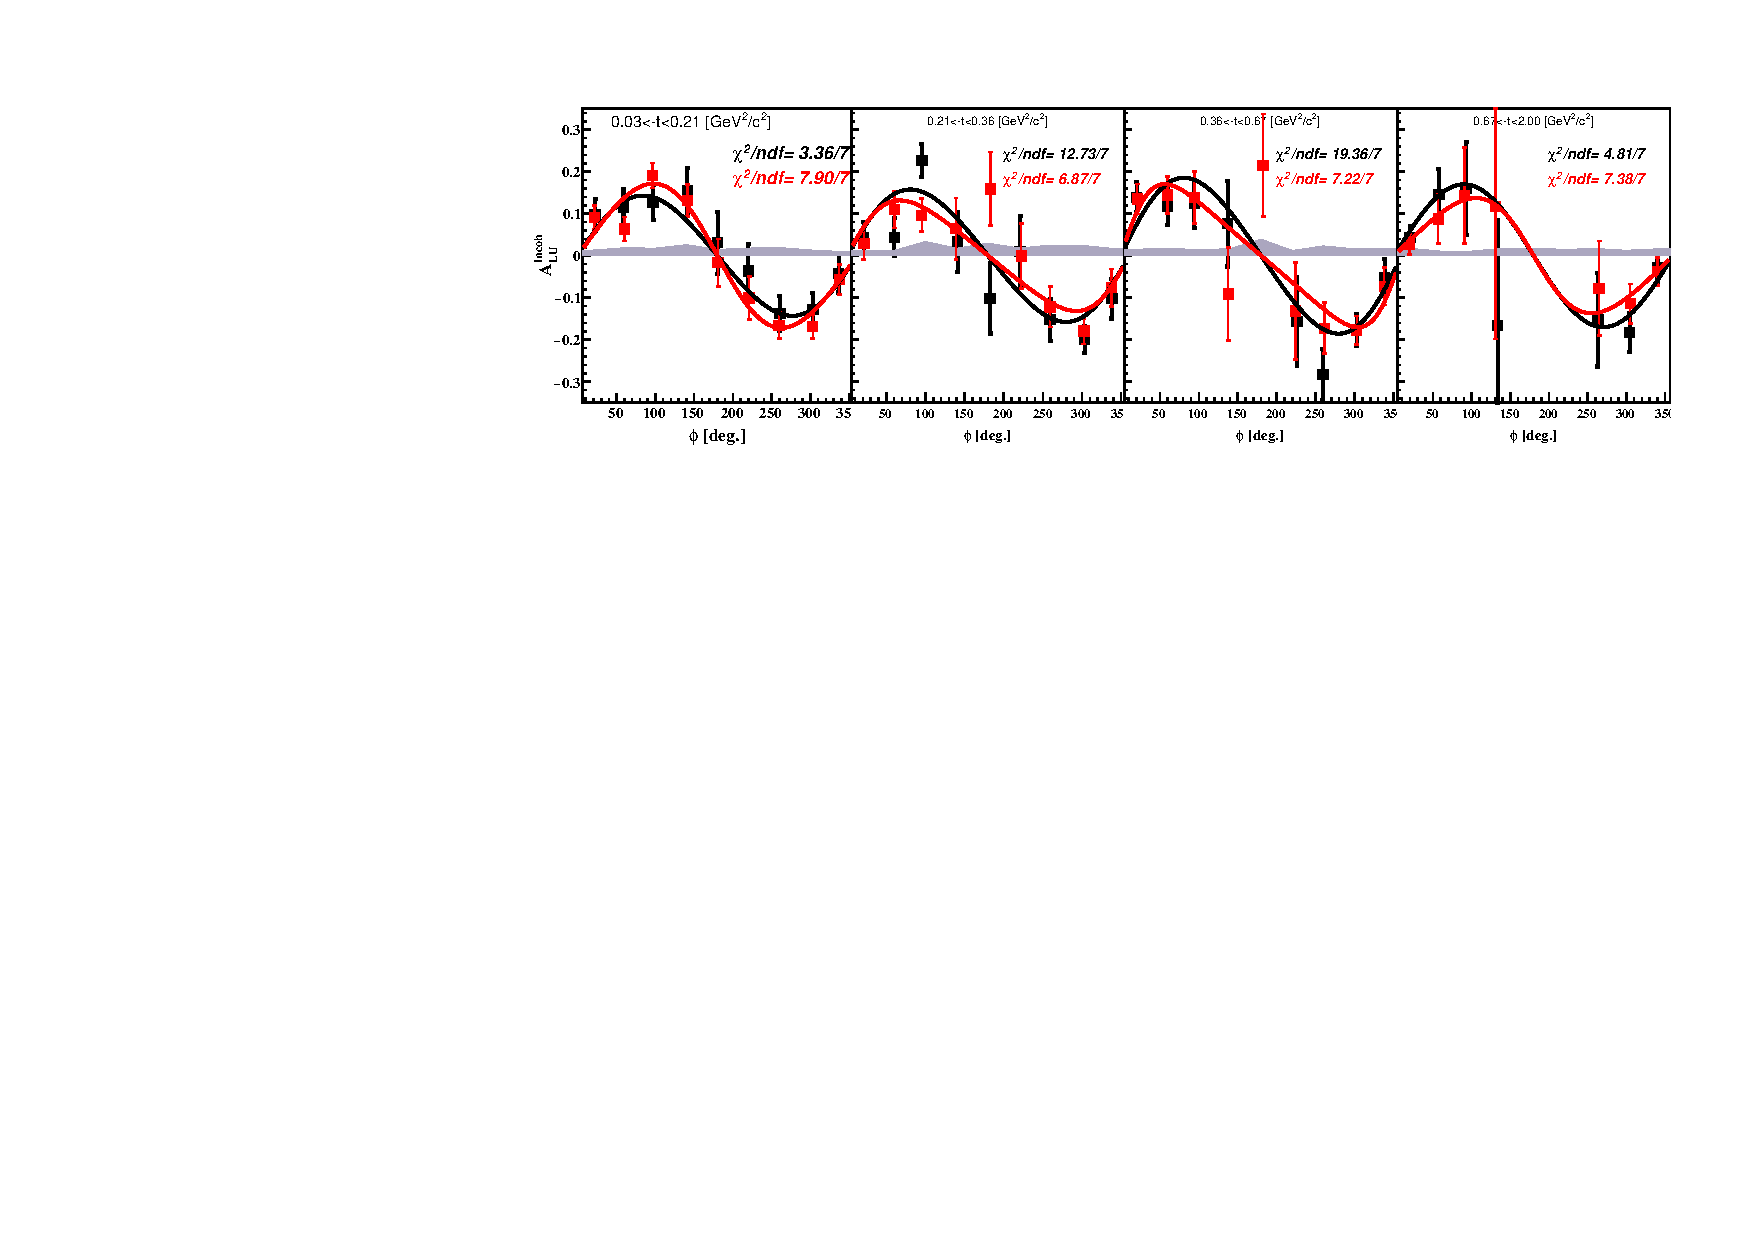
\includegraphics[width=15cm]{fig/ALU_phi_p_t.pdf}
\caption{The EG6 incoherent $A_{LU}$ as a function of $\phi$. Results are 
   presented for different $Q^{2}$ bins (top panel), $x_{B}$ bins (middle 
panel), and $t$ bins (bottom panel) using $t$ in black points and using the 
corrected $t'$ in red points.  The red curves are the results of our fits with 
the form $\frac{\alpha sin(\phi)}{1+ \beta cos(\phi)}$.}
\label{fig:alu}
\end{figure}

\begin{figure}[tb]
   \centering
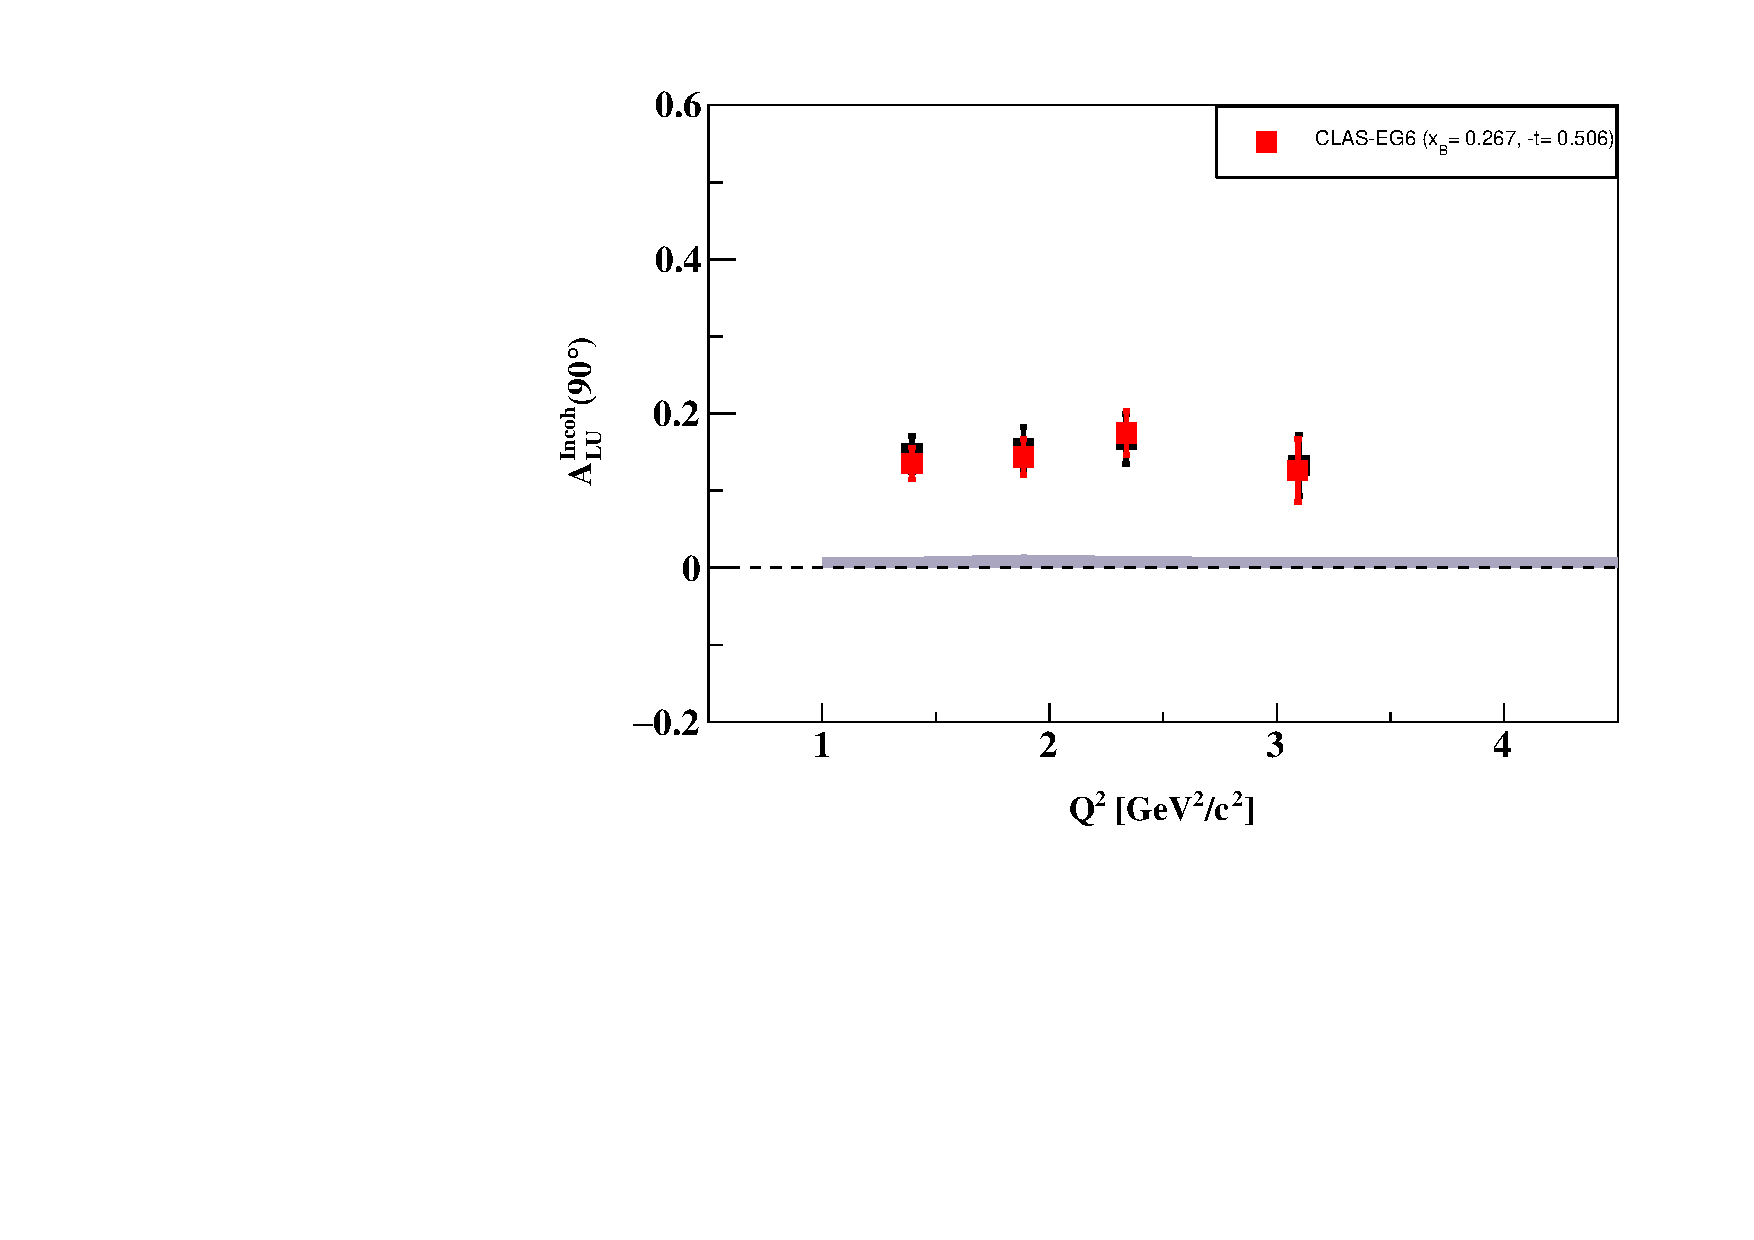
\includegraphics[width=12cm]{fig/ALU_90_p_vs_Q2_shortscenrario.pdf}
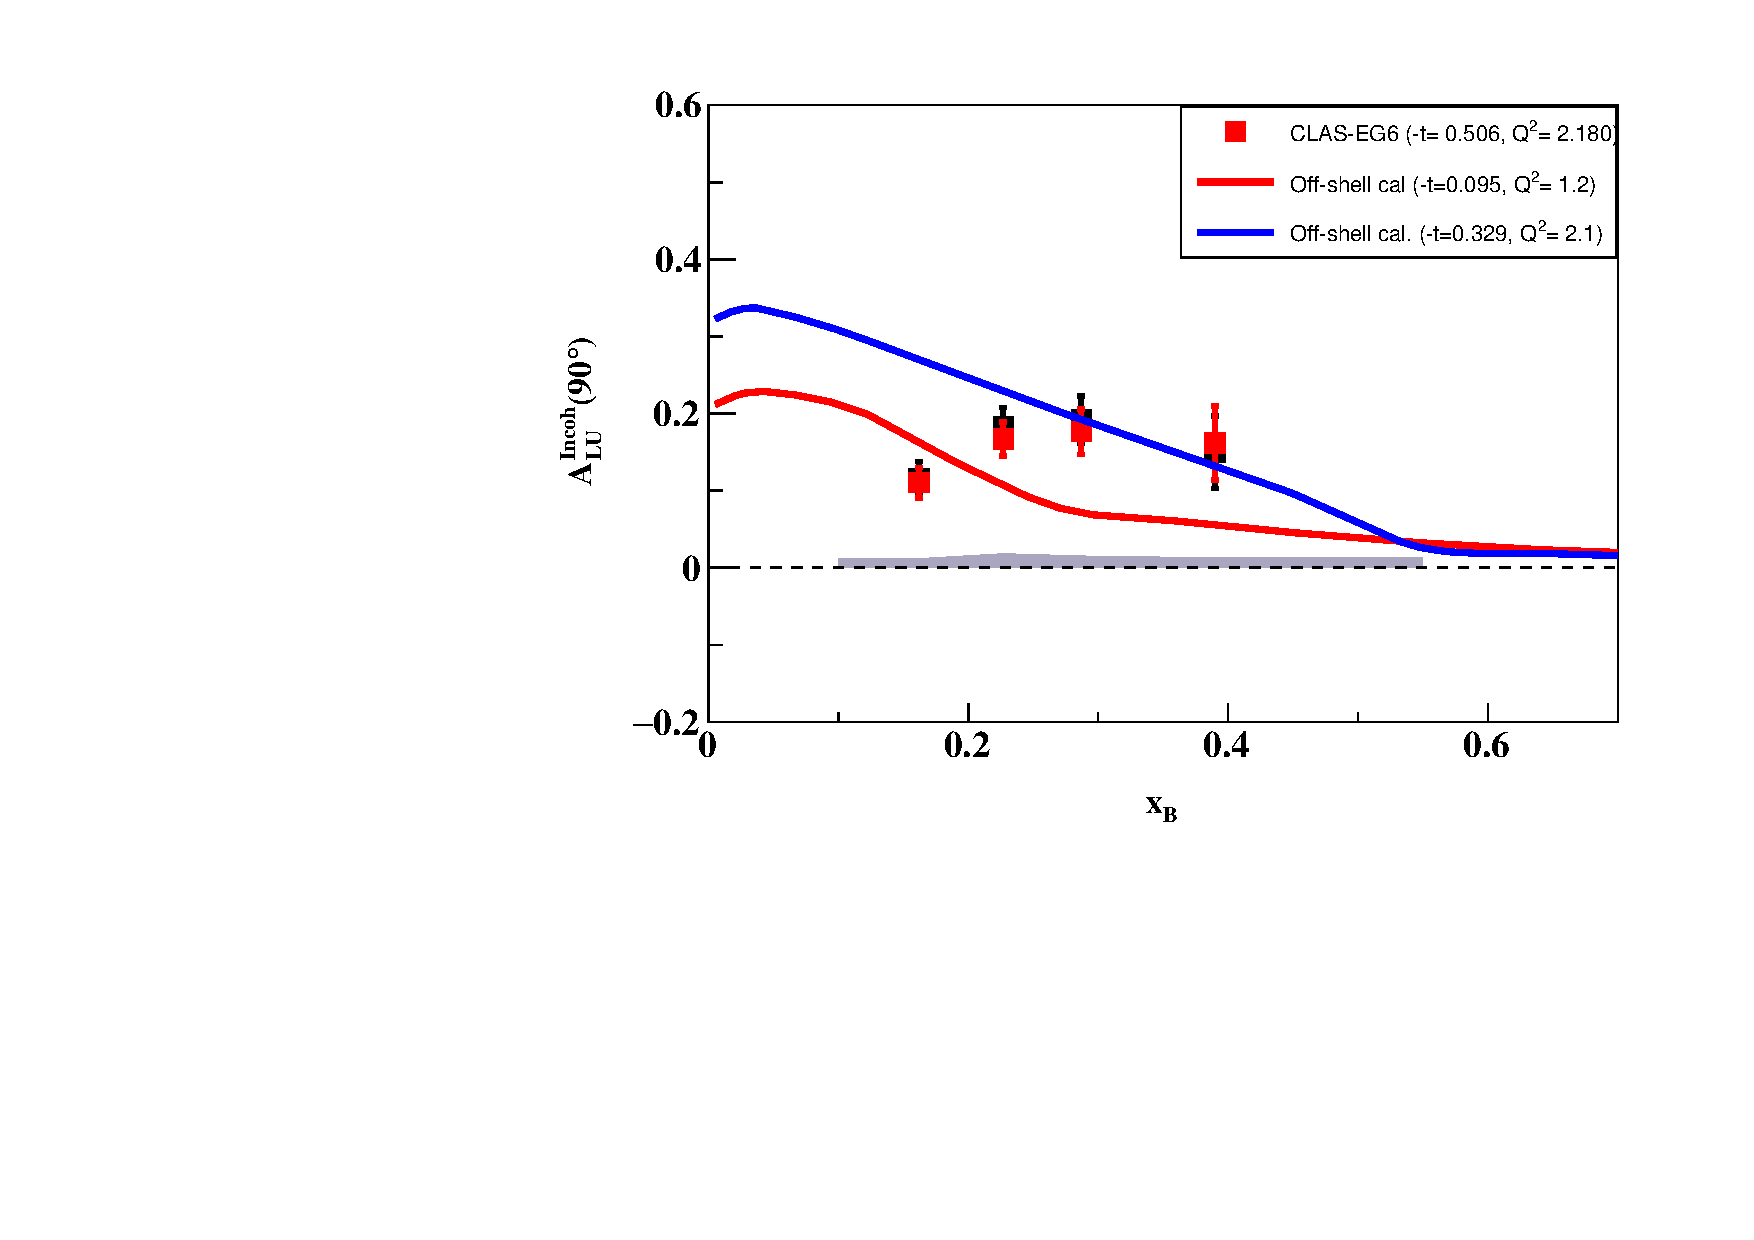
\includegraphics[width=12cm]{fig/ALU_90_p_vs_x_shortscenrario.pdf}
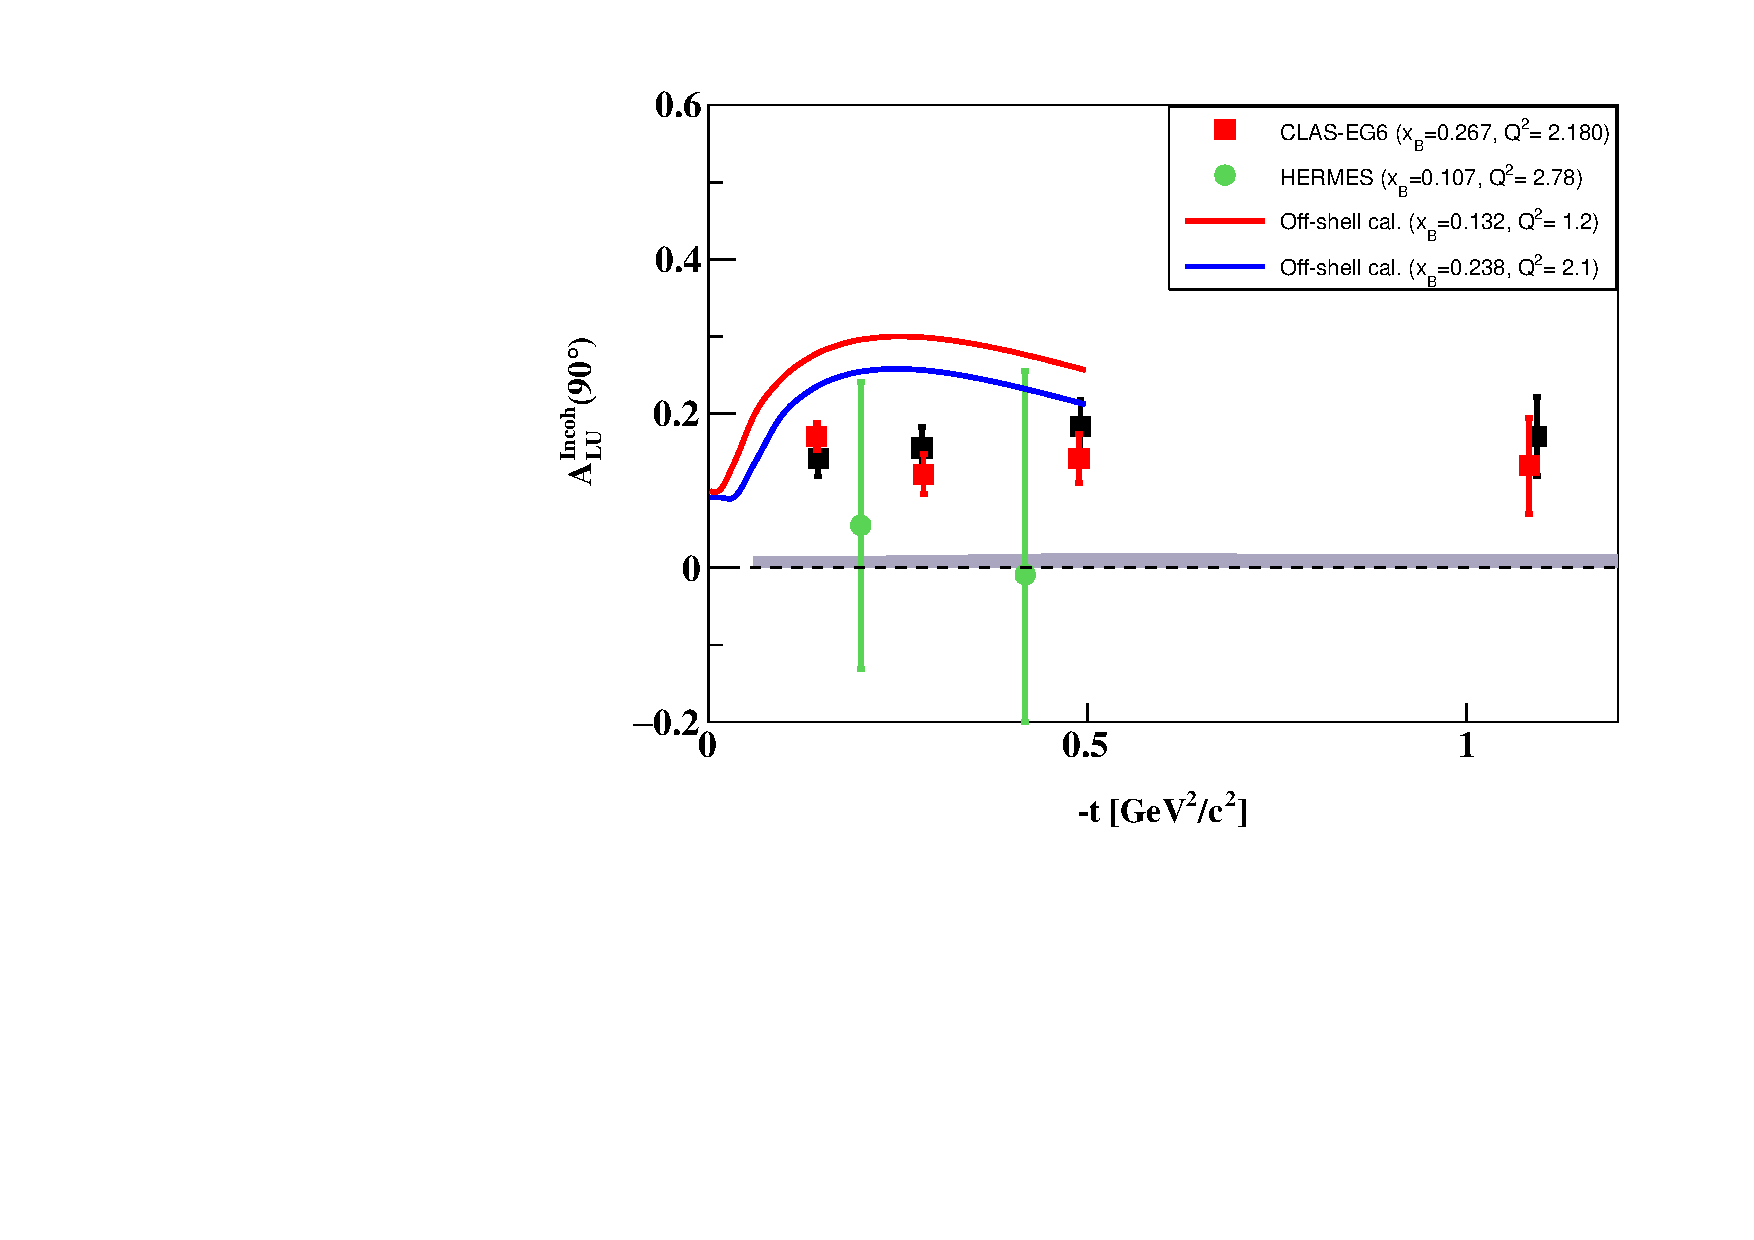
\includegraphics[width=12cm]{fig/ALU_90_p_vs_t_shortscenrario.pdf}
\caption{The EG6 incoherent $Q^{2}$ (left), $x_{B}$ (middle), and 
$t$-dependencies (right) of the $A_{LU}$ at $\phi$~=~90$^{\circ}$ using $t$ in 
black points and using the corrected $t'$ in red points. }
\label{fig:alu90}
\end{figure}




\section{Conclusions}
We improved the EG6 incoherent DVCS channel via the $t'$ that is calculated 
using the virtual and the final state real photons with corrections based on 
similar analysis on the free proton DVCS sample using the same setup of CLAS 
detector. The $Q^{2}$ and $x_B$ dependences of the asymmetries have shown 
slight changes using $t'$ rather than $t$, while the effect is bigger on the 
t-dependence, with overall changes are compatible with the statistical error 
bars.  Based on the free proton DVCS data, no induced systematic uncertainties 
are observed on the $Q^{2}$ and $x_B$, while some appear on $t$, which will be 
added to the EG6 incoherent asymmetries.

\end{document}
